%%%%%%%%%%%%%%%%%%%%%%%%%%%%%%%%%%%%%%%%%%%%%%%%%%%
%
%  New template code for TAMU Theses and Dissertations starting Spring 2021.  
%
%
%  Last Updated: 1/13/2021
%
%%%%%%%%%%%%%%%%%%%%%%%%%%%%%%%%%%%%%%%%%%%%%%%%%%%

% THIS TEMPLATE IS THE MOST
% CURRENT. SEE THE FILES README.TXT AND NEWCHANGES.TXT
% FOR MORE INFORMATION.

\documentclass[12pt]{report}

\usepackage{tamuconfig}


% Most of the packages that set the default settings
% for the document have moved to the style file
% tamuconfig.sty. This includes

%These next lines change the font. Fixes for certain
%fonts will be implemented in a future release.

%Comment this line if you do not wish to use Times
%New Roman. The font used will then be the LaTeX
%default of Computer Modern.
\usepackage{times}
%\usepackage{cmbright}
\usepackage[T1]{fontenc}

% For natbib-style references, uncomment this.
%\usepackage{natbib}

%This package allows for the use of graphics in the
%document.
\usepackage{graphicx}
\usepackage{pdflscape}
\usepackage{afterpage}

%If you have JPEG format images, add .jpg as an
%allowed file extension below. Same for Bitmaps (.bmp).
\DeclareGraphicsExtensions{.png}

%It is best practice to keep all your pictures in
%one folder inside the main directory in which your
%TeX file is kept. Here the folder is named "graphic."
%Replace the name here with your folder's name, if needed.
%The period is needed due to relative referencing.
\graphicspath{ {./graphic/} }

% For quick document navigation.
\usepackage{url}
\usepackage{breakurl}
\usepackage[hidelinks]{hyperref}
\usepackage{multirow}
	
\def\UrlBreaks{\do\/\do-}

%%%%%%%%%%%%%%%%%%%%%%%%%%%%%%%%%%%%%%%%%%%%%%%%%%%%%%%%%
%Please place all your personal packages here. Check to
%see if the packages you wish to use are not already
%declared above. Placing all your personal packages
%here allows me to determine if there are any package
%issues in compilation, as well as any conflicts
%that may arise by the order of loading.
%
%%%%%%%%%%%%%%%%%%%%%%%%%%%%%%%%%%%%%%%%%%%%%%%%%%%%%%%%%
%%%%%%%%%%%%%%%%%%%%%%%%%%%%%%%%%%%%%%%%%%%%%%%%%%%%%%%%%
%Begin student defined packages.
%%%%%%%%%%%%%%%%%%%%%%%%%%%%%%%%%%%%%%%%%%%%%%%%%%%%%%%%%


%%%%%%%%%%%%%%%%%%%%%%%%%%%%%%%%%%%%%%%%%%%%%%%%%%%%%%%%%
%End student defined packages.
%%%%%%%%%%%%%%%%%%%%%%%%%%%%%%%%%%%%%%%%%%%%%%%%%%%%%%%%%

% End preamble. Document begins below.
\begin{document}

%The title of your document goes here.
%Spacing may need to be adjusted if your title is long
%and pushes the copyright off the page.
\renewcommand{\tamumanuscripttitle}{A Domain-Specific Language Approach to Support Monitoring and Surveillance Within Wholesale Electricity Markets}


%Type only Thesis, Dissertation, or Record of Study.
\renewcommand{\tamupapertype}{Dissertation Proposal}

%Your full name goes here, as it is in university records. Check your student record on Howdy if there is any mismatch.
\renewcommand{\tamufullname}{Eric Charles Grasby}

%The degree title goes here. See the GPS site for more info.
\renewcommand{\tamudegree}{\MakeUppercase{Doctor of Philosophy}}
\renewcommand{\tamuchairone}{Dr. Daniel Berleant, Professor of Information Science}


% Uncomment out the next line if you have co-chairs.  You will also need to edit the titlepage.tex file.
%\newcommand{\tamuchairtwo}{Additional Chair Name}
\renewcommand{\tamumemberone}{Dr. Maria Gingras, Lead Market Monitor, Southwest Power Pool}
\newcommand{\tamumembertwo}{Dr. Elizabeth Pierce, Department Chair, Department of Information Science}
\newcommand{\tamumemberthree}{Dr. Ningning Wu, Professor of Information Science}
\renewcommand{\tamudepthead}{Dr. Elizabeth Pierce}

%Type only May, August, or December.
\renewcommand{\tamugradmonth}{August}
\renewcommand{\tamugradyear}{2026}
%Your department name goes here.
\renewcommand{\tamudepartment}{Department of Information Science}


%%%%%%%%%%%%%%%%%%%%%%%%%%%%%%%%%%%%%%%%%%%%%%%%%%%
%
%  New template code for TAMU Theses and Dissertations starting Spring 2021.  
%
%
%  Author: Thesis Office
%  
%  Last Updated: 1/13/20217
%
%%%%%%%%%%%%%%%%%%%%%%%%%%%%%%%%%%%%%%%%%%%%%%%%%%%

%%%%%%%%%%%%%%%%%%%%%%%%%%%%%% 
%% TITLE PAGE
%% The values get updated automatically.  Please do not make changes to this file other than adding/deleting committee members where necessary.
%%%%%%%%%%%%%%%%%%%%%%%%%%%%%%

\providecommand{\tabularnewline}{\\}



\begin{titlepage}
\begin{center}
\begin{doublespace}

\MakeUppercase{  \tamumanuscripttitle}
\end{doublespace}
\vspace{4em}

A \tamupapertype

by

\MakeUppercase{\tamufullname}

\vspace{2em}

\begin{singlespace}

Submitted to the Graduate School \\
University of Arkansas at Little Rock \\

in partial fulfillment of the requirements for the degree of \\
\end{singlespace}

\MakeUppercase{\tamudegree} \\
in Computer and Information Sciences (CIS) \\
Information Quality Track
\par\end{center}
\vspace{1em}
\begin{doublespace}

\end{doublespace}
\begin{tabular}{ll}
 & \tabularnewline
& \cr
% If you have Co-Chairs comment out the 'Chair of Committee' line below and uncomment the 'Co-Chairs of Committee' line.
Chair of Committee, & \tamuchairone\tabularnewline
%Co-Chairs of Committee, & \tamuchairone\tabularnewline & \tamuchairtwo\tabularnewline
Committee Members, & \tamumemberone\tabularnewline
 & \tamumembertwo\tabularnewline
 & \tamumemberthree\tabularnewline
%Head of Department, & \tamudepthead\tabularnewline

\end{tabular}

\vspace{3em}

\begin{center}
%\tamugradmonth \hspace{2pt} \tamugradyear%
September 2025

\vspace{1em}

\tamudepartment \par
\vspace{1em}
%Copyright \tamugradyear \hspace{.5em}\tamufullname%
M.S., Information Quality, UA Little Rock, 2020.\\
G.C., Information Quality, UA Little Rock, 2020.\\
B.S., Information Science, UA Little Rock, 2018.\\
\par\end{center}
\end{titlepage}
\pagebreak{}




 % This is simply a file that formats and adds your titlepage, please do not edit this unless you have a specific need. .
%%%%%%%%%%%%%%%%%%%%%%%%%%%%%%%%%%%%%%%%%%%%%%%%%%%
%
%  New template code for TAMU Theses and Dissertations starting Spring 2021.  
%
%
%  Author: Thesis Office
%  
%  Last Updated: 1/13/2021
%
%%%%%%%%%%%%%%%%%%%%%%%%%%%%%%%%%%%%%%%%%%%%%%%%%%%

%%%%%%%%%%%%%%%%%%%%%%%%%%%%%%%%%%%%%%%%%%%%%%%%%%%%%%%%%%%%%%%%%%%%%%
%%                           SECTION I
%%%%%%%%%%%%%%%%%%%%%%%%%%%%%%%%%%%%%%%%%%%%%%%%%%%%%%%%%%%%%%%%%%%%%


\pagestyle{plain} % No headers, just page numbers
\pagenumbering{roman} % roman numerals
\addcontentsline{toc}{chapter}{APPROVAL}
\setcounter{page}{1}

\noindent This dissertation \textbf{proposal}, "\tamumanuscripttitle", by Eric Charles Grasby, is approved by:

\begin{table}[h]
    \centering
    \begin{tabularx}{\textwidth}{X X}
        \vspace{16pt}
        Dissertation Advisor: \\ & \hline \newline Dr. Daniel Berleant \newline Professor of Information Science \\
        \vspace{16pt}
        Co-Advisor: \\ & \hline \newline Dr. Maria Gingras \newline Lead Market Monitor, SPP  \\
        \vspace{16pt}
        Dissertation Committee:  \\ & \hline \newline Dr. Elizabeth Pierce \newline Professor of Information Science \\
        \vspace{16pt}
        \hfill \\ & \hline \newline Dr. Ningning Wu \newline Professor of Information Science  \\
        \vspace{16pt}
        Program Coordinator: \\ & \hline \newline Dr. John Talburt \newline Acxiom Chair of Information Quality \\
        \vspace{16pt}
        Graduate Dean: \\ & \hline \newline Dr. Brian Berry \newline Professor of Chemistry
        \vspace{1pt}
    \end{tabularx}
\end{table}

\begin{center}
    \textit{This page is intentionally retained for inclusion in the final dissertation}
\end{center}

\pagebreak{}
%%%%%%%%%%%%%%%%%%%%%%%%%%%%%%%%%%%%%%%%%%%%%%%%%%%
%
%  New template code for TAMU Theses and Dissertations starting Spring 2021.  
%
%
%  Author: Thesis Office
%  
%  Last Updated: 1/13/2021
%
%%%%%%%%%%%%%%%%%%%%%%%%%%%%%%%%%%%%%%%%%%%%%%%%%%%
%%%%%%%%%%%%%%%%%%%%%%%%%%%%%%%%%%%%%%%%%%%%%%%%%%%%%%%%%%%%%%%%%%%%%
%%                           ABSTRACT 
%%%%%%%%%%%%%%%%%%%%%%%%%%%%%%%%%%%%%%%%%%%%%%%%%%%%%%%%%%%%%%%%%%%%%

\chapter*{ABSTRACT}
\addcontentsline{toc}{chapter}{ABSTRACT} % Needs to be set to part, so the TOC doesn't add 'CHAPTER ' prefix in the TOC.

\pagestyle{plain} % No headers, just page numbers
\pagenumbering{roman} % Roman numerals
\setcounter{page}{2}

\indent This dissertation investigates an intersection between multiple domains of expertise related to electric markets and electric market monitoring. These domains are: 1) data and information quality, 2) language engineering, and 3) knowledge management. Electricity markets present unique opportunities for deriving new value from data and information assets, due to the enormous volume of data generated, each day, by public utilities, transmission and market operators, and regulators. These data assets are critically necessary to both ensuring reliable operation of the North American Bulk Electric System (BES), as well as operating efficient markets for selling energy on a wholesale scale. The outcomes of these markets have tangible, long-term impacts on system reliability, prices for residential and commercial energy consumers, and electricity infrastructure development. 
%%TODO: 2025-06-27 - reword "that the BES remains..." to refer to the market on top of the BES instead. This is in the Introduction chapter too.
Due to the complex nature of energy marketplaces, there are abundant opportunities for market participants to manipulate these markets. Market monitors are the professionals who work to ensure that the markets utilizing the BES remain fair, efficient, and open-access in the face of such manipulative actions. They perform routine surveillance and forensic analysis to identify instances of fraud and market manipulation and refer such cases to regulatory authorities. 

This research investigates the efficacy of designing and implementing a layer of abstraction between market monitors and the data that they use to perform their forensic analysis. Using domain-specific programming language engineering and information quality principles, the intent is to develop a system to ease data manipulation for market monitors.

\pagebreak{}

%%%%%%%%%%%%%%%%%%%%%%%%%%%%%%%%%%%%%%%%%%%%%%%%%%%%
%
%  New template code for TAMU Theses and Dissertations starting Spring 2021.  
%
%
%  Author: Thesis Office
%  
%  Last Updated: 1/13/2021
%
%%%%%%%%%%%%%%%%%%%%%%%%%%%%%%%%%%%%%%%%%%%%%%%%%%%

%%%%%%%%%%%%%%%%%%%%%%%%%%%%%%%%%%%%%%%%%%%%%%%%%%%%%%%%%%%%%%%%%%%%%%
%%                           DEDICATION
%%%%%%%%%%%%%%%%%%%%%%%%%%%%%%%%%%%%%%%%%%%%%%%%%%%%%%%%%%%%%%%%%%%%%
\chapter*{DEDICATION}
\addcontentsline{toc}{chapter}{DEDICATION}  % Needs to be set to part, so the TOC doesnt add 'CHAPTER ' prefix in the TOC.

\begin{center}
\vspace*{\fill}
\noindent \textit{I attempted suicide, in 2022, in the wake of a devastating personal event. I am thankful that it was an attempt that ended in failure. For my true friends Jacob and Meredith Tillman (née Ashley), you will always have my gratitude for saving my life.}

\vspace*{\fill}

\noindent \textit{If I can name one thing that pulled me through the years following that experience, it would be my family. It would constitute an absurd lack of devotion on my part to dedicate this dissertation to anyone other than them. My parents have shown my siblings and I nothing but love in our lives. For as much as I earned this achievement, I earned it to share with the Grasby family.}

\vspace*{\fill}

\noindent \textit{For my parents, Tina and Charles. For my sister, Madasyn. For my brother and sister-in-law, Robert, Brittany (and my nephews, Miles and Maddox). For my cousin, David Parker. For my grandmother, Louise. For my late grandparents, Hubert and Addie Mae. For my maternal, late, grandfather that I never got the chance to meet, Desi Sandoval. For my paternal uncle, Leonard. And for a true family friend that died too young, Doug Durham. I am glad that I am still here to share this life with each of you. Any benefit that this research brings to society: I dedicate to you.}

\vspace*{\fill}

\noindent \textit{Furthermore, I want to extend the family metaphor. For anyone that reads this- any human- that has struggled with their mental health, their identity, or finding their place in the world: I understand. I have been there. We are all in this together. This achievement is for you, too.}

\vspace*{\fill}

\noindent \textit{And, finally, to both Miss Natasha and Rebecca- thank you, both, for changing my life (albeit in fundamentally different ways).}
\end{center}

\pagebreak{}%
%%%%%%%%%%%%%%%%%%%%%%%%%%%%%%%%%%%%%%%%%%%%%%%%%%%%
%
%  New template code for TAMU Theses and Dissertations starting Fall 2016.  
%
%
%  Author: Thesis Office
%  
%  Last Updated: 1/13/2021
%
%%%%%%%%%%%%%%%%%%%%%%%%%%%%%%%%%%%%%%%%%%%%%%%%%%%


%%%%%%%%%%%%%%%%%%%%%%%%%%%%%%%%%%%%%%%%%%%%%%%%%%%%%%%%%%%%%%%%%%%%%%
%%                           ACKNOWLEDGMENTS
%%%%%%%%%%%%%%%%%%%%%%%%%%%%%%%%%%%%%%%%%%%%%%%%%%%%%%%%%%%%%%%%%%%%%
\chapter*{ACKNOWLEDGMENTS}
\addcontentsline{toc}{chapter}{ACKNOWLEDGMENTS}  % Needs to be set to part, so the TOC doesnt add 'CHAPTER ' prefix in the TOC.

Many people lent me their support during the development of this dissertation, and I am very happy to acknowledge them here. My sincere thanks go to my research advisors, Dr. Daniel Berleant and Dr. Maria Gingras. Both took an interest in me and helped shape my ideas for this research. 

Dr. Berleant has been an instructor to me since the days of my undergraduate degree. I am glad to have had the opportunity to perform my first, rigorous research project under a professional of his calibur.

Dr. Gingras (Maria) is both a professional and personal mentor to me, and I am thankful that she lent her time to become an affiliate faculty member of UA Little Rock and join my dissertation committee. Maria is a wealth of knowledge in the market monitoring discipline, and her instruction, mentorship, and encouragement have made a tremendous difference in my life.

My thanks also goes to the other members of my dissertation committee, Dr. Elizabeth Pierce and Dr. Ningning Wu. Your guidance throughout my academic career has been nothing short of a blessing. I also must thank Dr. John Talburt, whom encouraged me to join the information quality program at UA Little Rock many years ago. 

Finally, I want to acknowledge the contributions of my co-workers and friends within the market monitoring unit at Southwest Power Pool. Many of my colleagues in the MMU have lent their expertise to help me succeed in my work, and I couldn't have completed my dissertation without their support. Special thanks go to both my best friend and colleague, Mark Rouse, and my manager, Raleigh Mohr. Mark has been a steadfast friend in my career, and Raleigh has been an incredibly supportive mentor. I am thankful to acknowledge their help as I completed this program.

\pagebreak{}%
%%%%%%%%%%%%%%%%%%%%%%%%%%%%%%%%%%%%%%%%%%%%%%%%%%%%
%
%  New template code for TAMU Theses and Dissertations starting Spring 2021.  
%
%
%  Author: Thesis Office
%  
%  Last Updated: 1/13/2021
%
%%%%%%%%%%%%%%%%%%%%%%%%%%%%%%%%%%%%%%%%%%%%%%%%%%%


%%%%%%%%%%%%%%%%%%%%%%%%%%%%%%%%%%%%%%%%%%%%%%%%%%%%%%%%%%%%%%%%%%%%%%
%%             CONTRIBUTORS AND FUNDING SOURCES
%%%%%%%%%%%%%%%%%%%%%%%%%%%%%%%%%%%%%%%%%%%%%%%%%%%%%%%%%%%%%%%%%%%%%
\chapter*{CONTRIBUTORS AND FUNDING SOURCES}
\addcontentsline{toc}{chapter}{CONTRIBUTORS AND FUNDING SOURCES}  % Needs to be set to part, so the TOC doesn't add 'CHAPTER ' prefix in the TOC.


%This section is taken directly from the MS Word templates.

%Old version below.

%All theses and dissertations must include a contributors and funding sources section. In this section, name all members of the dissertation committee, and any collaboration with others in carrying out your thesis or dissertation research. Your independent contributions must be made clear.
%
%If financial support from the university or any other source was gained to conduct your thesis or dissertation research and compilation, it must be listed in this section. If you completed all work independently without outside financial support, indicate this here.
%\textit{(Sample Wording)}
%
%This work was supported by a dissertation committee consisting of Professor XXX [advisor – also note if co-advisor] and XXXX of the Department of [Home Department] and Professor(s) XXXX of the Department of [Outside Department].
% 
%The data analyzed for Chapter III was provided by Professor XXXX. The analyses depicted in Chapter IV were conducted in part by Rebekah Jones of the Department of Bio-statistics and were published in (year) in an article listed in the Biographical Sketch. 
%
%All other work conducted for the dissertation was completed by the student independently.
%
%\noindent \textit{(or)}
%
%This work was supervised by a dissertation committee consisting of Professor XXXX [advisor – also note if co-advisor] and Professor(s) XXXX of the Department of [Home Department] and Professor(s) XXXX of [Outside Department]. All work for the dissertation was completed independently by the student.
%
%\noindent \textit{(or)}
%
%Graduate study was supported by a fellowship from Texas A\&M University and a dissertation research fellowship from XXX Foundation.

\subsection*{Contributors}
This work was supported by a thesis (or) dissertation committee consisting of Professor Jane Doe [advisor --– also note if co-advisor] and John Doe of the Department of [Home Department] and Professor(s) XXXX of the Department of [Other Department].

The data analyzed for Chapter IV was provided by Professor Thompson. The analyses depicted in Chapter X were conducted in part by Daniel James of the Department of Statistics and were published in (2004) in an article listed in the Journal of Things.

All other work conducted for the thesis (or) dissertation was completed by the student independently.
\subsection*{Funding Sources}
Graduate study was supported by a fellowship from Texas A\&M University and a dissertation research fellowship from That Foundation. OR No other outside source of funding was provided. One or the other must be stated.
\pagebreak{}
%%%%%%%%%%%%%%%%%%%%%%%%%%%%%%%%%%%%%%%%%%%%%%%%%%%
%
%  New template code for TAMU Theses and Dissertations starting Spring 2021.  
%
%
%  Author: Thesis Office
% 
%  Last Updated: 1/13/2021
%
%%%%%%%%%%%%%%%%%%%%%%%%%%%%%%%%%%%%%%%%%%%%%%%%%%%

%%%%%%%%%%%%%%%%%%%%%%%%%%%%%%%%%%%%%%%%%%%%%%%%%%%%%%%%%%%%%%%%%%%%%%
%%                           NOMENCLATURE
%%%%%%%%%%%%%%%%%%%%%%%%%%%%%%%%%%%%%%%%%%%%%%%%%%%%%%%%%%%%%%%%%%%%%

\chapter*{INDUSTRY ACRONYMS} \label{nomenclature}
\addcontentsline{toc}{chapter}{INDUSTRY ACRONYMS}  % Needs to be set to part, so the TOC doesnt add 'CHAPTER ' prefix in the TOC.

%A note about aligning: These entries will align
%themselves according to the ampersand (&).
%No extra spaces are needed, as seen in some of
%the entries below.

%Example of the longtable environment.
\hspace*{-1.25in}
\vspace{12pt}
\begin{spacing}{1.0}
	\begin{longtable}[htbp]{@{}p{0.35\textwidth} p{0.62\textwidth}@{}}
	   % \begin{tabular}{@{}p{0.33\textwidth} p{0.62\textwidth}@{}}
        APAC & Asian-Pacific Region \\ [0.5ex]
	AS & Ancillary Services \\ [0.5ex]
        BES	& Bulk Electric System \\ [0.5ex]
        BSS & Bilateral Settlement Schedule \\ [0.5ex]
        CRM & Capacity Reserve Margin \\ [0.5ex]
        DA & Day-Ahead Market \\ [0.5ex]
        DSL & Domain-Specific Language \\ [0.5ex]
        DSRM & Design Science Research Methodology \\ [0.5ex]
        DQ & Data Quality \\ [0.5ex]
        EMEA & Europe, the Middle-East, and Africa region \\ [0.5ex]
        ETL & Extract-Transform-Load \\ [0.5ex]
        FERC & Federal Energy Regulatory Commission \\ [0.5ex]
        GPL & General-Purpose Language \\ [0.5ex]
        HHI & Herfindahl-Hirschman Index \\ [0.5ex]
        IQ & Information Quality \\ [0.5ex]
        ISO & Independent System Operator \\ [0.5ex]
        LMP & Locational Marginal Price \\ [0.5ex]
        MMU & Market Monitoring Unit \\ [0.5ex]
        MP & Market Participant \\ [0.5ex]
        MW & Megawatt \\ [0.5ex]
        NERC & North-American Energy Reliability Corporation \\ [0.5ex]
	RTO & Regional Transmission Organization \\	[0.5ex] %[2ex] provides double space between each row
        RT & Real-Time Market \\ [0.5ex]
        SME & Subject Matter Expert \\ [0.5ex]
        SOX & Sarbanes-Oxley Act of 2002 \\ [0.5ex]
        TCR / FTR & Transmission Congestion / Financial Transmission Rights \\ [0.5ex]
        TO / TOP & Transmission Owner / Transmission Operator \\ [0.5ex]
		%XXXXXXXX		&	This is an optional page. Random word to test how long the sentence can be? This is just for test purpose. The current setting aims to align left/right margin same as all other pages.\\	[2ex]
	   % \end{tabular}%
	\end{longtable}
\end{spacing}

\pagebreak{}

%%%%%%%%%%%%%%%%%%%%%%%%%%%%%%%%%%%%%%%%%%%%%%%%%%%
%
%  New template code for TAMU Theses and Dissertations starting Spring 2021.  
%
%
%  Author: Thesis Office
% 
%  Last Updated: 1/13/2021
%
%%%%%%%%%%%%%%%%%%%%%%%%%%%%%%%%%%%%%%%%%%%%%%%%%%%
%%%%%%%%%%%%%%%%%%%%%%%%%%%%%%%%%%%%%%%%%%%%%%%%%%%%%%%%%%%%%%%%%%%%%%
%%       TABLE OF CONTENTS
%%%%%%%%%%%%%%%%%%%%%%%%%%%%%%%%%%%%%%%%%%%%%%%%%%%%%%%%%%%%%%%%%%%%%
% single-space sections in Table of Contents  - commented in version 1.7
%\renewcommand{\cftsecafterpnum}{\vskip0.5\baselineskip}
%\renewcommand{\cftsubsecafterpnum}{\vskip0.5\baselineskip}
%\renewcommand{\cftsubsubsecafterpnum}{\vskip0.5\baselineskip}
%%%%%%%%%%%%%%%%%%%%%%%%%%%%%%%%%%%%%%%%%%%%%%%%%%%

\phantomsection
\addcontentsline{toc}{chapter}{TABLE OF CONTENTS}  

\begin{singlespace}
\renewcommand\contentsname{\normalfont} {\centerline{TABLE OF CONTENTS}}

\setcounter{tocdepth}{4} % This puts \subsubsection[]{×} in your List of Tables.  The default is 3.


%%%%%%%%%%%%%  Adds Page above the page number in TOC
\setlength{\cftaftertoctitleskip}{1em}
\renewcommand{\cftaftertoctitle}{%
\hfill{\normalfont {Page}\par}}


\tableofcontents

%\addtocontents{toc}{\protect\afterpage{~\hfill\normalfont{Page}\par\medskip}}
\end{singlespace}

\pagebreak{}

%%%%%%%%%%%%%%%%%%%%%%%%%%%%%%%%%%%%%%%%%%%%%%%%%%%%%%%%%%%%%%%%%%%%%%
%%                           LIST OF FIGURES
%%%%%%%%%%%%%%%%%%%%%%%%%%%%%%%%%%%%%%%%%%%%%%%%%%%%%%%%%%%%%%%%%%%%%

\phantomsection
\addcontentsline{toc}{chapter}{LIST OF FIGURES}  

\renewcommand{\cftloftitlefont}{\center\normalfont\MakeUppercase}

\setlength{\cftbeforeloftitleskip}{-12pt} %% Positions the LOF title vertically to match the chapter titles
\renewcommand{\cftafterloftitleskip}{12pt}


\renewcommand{\cftafterloftitle}{%
\\[4em]\mbox{}\hspace{2pt}FIGURE\hfill{\normalfont Page}\vskip\baselineskip}

\begingroup


\begin{center}
\begin{singlespace}
%% These values make the lof table entries appear double spaced between.
\setlength{\cftbeforechapskip}{0.4cm}
\setlength{\cftbeforesecskip}{0.30cm}
\setlength{\cftbeforesubsecskip}{0.30cm}
\setlength{\cftbeforefigskip}{0.4cm}
\setlength{\cftbeforetabskip}{0.4cm}

% Provided by Andy Philips.
% needed to make chapter gaps look no different than sections:
% \addtocontents{lof}{\protect\renewcommand*\protect\addvspace[1]{}}

% Philips' document had 30 figures. Is there a maximum number of figures
% that changes the spacing to non-uniform, i.e., not double-spaced
% between all entries?

\listoffigures

\end{singlespace}
\end{center}

\pagebreak{}


%%%%%%%%%%%%%%%%%%%%%%%%%%%%%%%%%%%%%%%%%%%%%%%%%%%%%%%%%%%%%%%%%%%%%%
%%                           LIST OF TABLES
%%%%%%%%%%%%%%%%%%%%%%%%%%%%%%%%%%%%%%%%%%%%%%%%%%%%%%%%%%%%%%%%%%%%%%
%
\phantomsection
\addcontentsline{toc}{chapter}{LIST OF TABLES}  

\renewcommand{\cftlottitlefont}{\center\normalfont\MakeUppercase}

\setlength{\cftbeforelottitleskip}{-12pt} %% Positions the LOT title vertically to match the chapter titles

%Note that the similar parameter in the LOF is 12pt; this
%is intentional to make the spacing between the headers
%and the first entry look consistent.
\renewcommand{\cftafterlottitleskip}{1pt}


\renewcommand{\cftafterlottitle}{%
\\[4em]\mbox{}\hspace{2pt}TABLE\hfill{\normalfont Page}\vskip\baselineskip}

\begin{center}
\begin{singlespace}

%% These values make the lot table entries appear double spaced between.
\setlength{\cftbeforechapskip}{0.4cm}
\setlength{\cftbeforesecskip}{0.30cm}
\setlength{\cftbeforesubsecskip}{0.30cm}
\setlength{\cftbeforefigskip}{0.4cm}
\setlength{\cftbeforetabskip}{0.4cm}

\listoftables 

\end{singlespace}
\end{center}
\endgroup
\pagebreak{}  % Need this for the page numbering to be correct.   % This is simply a file that formats and adds your toc, lof, and lot, please do not edit this unless you have a specific need.

%This section includes the individual chapters
%%%%%%%%%%%%%%%%%%%%%%%%%%%%%%%%%%%%%%%%%%%%%%%%%%%
%
%  New template code for TAMU Theses and Dissertations starting Spring 2021.  
%
%
%  Author: Thesis Office
%  
%  Last Updated: 1/13/2021
%
%%%%%%%%%%%%%%%%%%%%%%%%%%%%%%%%%%%%%%%%%%%%%%%%%%%

%%%%%%%%%%%%%%%%%%%%%%%%%%%%%%%%%%%%%%%%%%%%%%%%%%%%%%%%%%%%%%%%%%%%%%
%%                           SECTION I
%%%%%%%%%%%%%%%%%%%%%%%%%%%%%%%%%%%%%%%%%%%%%%%%%%%%%%%%%%%%%%%%%%%%%


\pagestyle{plain} % No headers, just page numbers
\pagenumbering{arabic} % Arabic numerals
\setcounter{page}{1}


\chapter{\uppercase {Introduction}}
\label{cha:Introduction}
This dissertation intends to introduce information quality research into the electricity market monitoring industry- a regulatory component of the North American Bulk Electric System (BES) \cite{ferc1} and their corresponding electric markets. Often touted as the "world's largest machine" \cite{stenvignils} by electrical industry staff, the BES has become an important dependency in the lives of virtually every resident of the United States, Canada, and (a portion of) Mexico.

To illustrate the opportunity that superimposing information quality research onto the market monitoring domain poses, this chapter shall introduce the concepts of the BES, electric markets, and Market Monitoring, and provide detail as to how applying information quality concepts to Market Monitoring will help serve a previously unsolved problem within the industry.

\section{The North American Bulk Electric System}

The BES \footnote{The North American Electric Reliability Corporation (NERC) serves as the Electric Reliability Operator (ERO) for the BES. In their Glossary of Terms (see References section), the BES refers to all high-voltage transmission lines and substations, generation resources, and all other equipment used in both inter/intra-state transmission of electric capacity.}
is a highly integrated system that facilitates transmission of electric power (generalized as “energy”) from generation to energy consumption (generalized as a “load”) in a real-time and balanced \footnote{The term “balancing” refers to the need to only generate power as it is needed for consumption- subject to system capacity and economic constraints.}
manner. With few (relatively recent) exceptions \footnote{Storage resources are a developing technology that can store energy for deployment during reliability emergencies or intervals of energy scarcity.}
, energy is not stored in the system; it is generated (in response to a demand forecast) and then immediately transmitted and consumed by various loads. Figure \ref{fig:BES_1} shows a conceptual configuration of some of the components \footnote{An important distinction to note is between the \textit{utility} and \textit{retail} sectors shown in Figure \ref{fig:BES_1}. While referred to by several names (i.e. wholesale), utility generation and transmission refers to bulk energy (on the scale of MW) that is transmitted on the BES. The retails sector involves distribution of energy to residences and low consumption (on the scale of kW) commercial enterprises. This research focuses on wholesale energy markets, and thus is concerned with the bulk power generation and transmission domains.}
involved in the operation of the BES. \cite{devasia}

The BES must be precisely managed, at all times, to balance power across the system and to serve load. Deviations can cause significant damage to BES infrastructure, as were seen during the February 2021 Winter Storm in Texas' electric grid \cite{balancing1}.
No one entity manages the entire BES. Instead, this job is shared across geographic locales. This paper focuses specifically on support for organized markets, which pool resources managed by a Regional Transmission Organization (RTO) or an Independent System Operator (ISO). These entities serve multiple roles; their primary role is to function as a grid operator. These organizations commit and dispatch electric generation (a coal plant or a wind farm, for example) based on the principle of security-constrained economic dispatch (SCED)
\footnote{Economic dispatch ("ED") is a concept that blends economics and the physical reality of the electric grid.}.

These organizations also frequently act as Reliability Coordinators (RC) and Balancing Authorities (BA), monitoring power flows, balancing the grid, and acting to restore system reliability during and after an emergency. One such function provided by BAs includes corrective frequency response. Many lay-persons are likely aware that the US electric grid operates, synchronously, at 60 Hz (or, 60 cycles per second). On such a broad scale, the collection of companies and regulation entities that operate the grid must also ensure minimal deviation from this baseline of 60 Hz. A broader engineering discourse of the electric generation and reliability functions of the BES is outside of the scope of this work.

\begin{figure}
\centering
\fbox{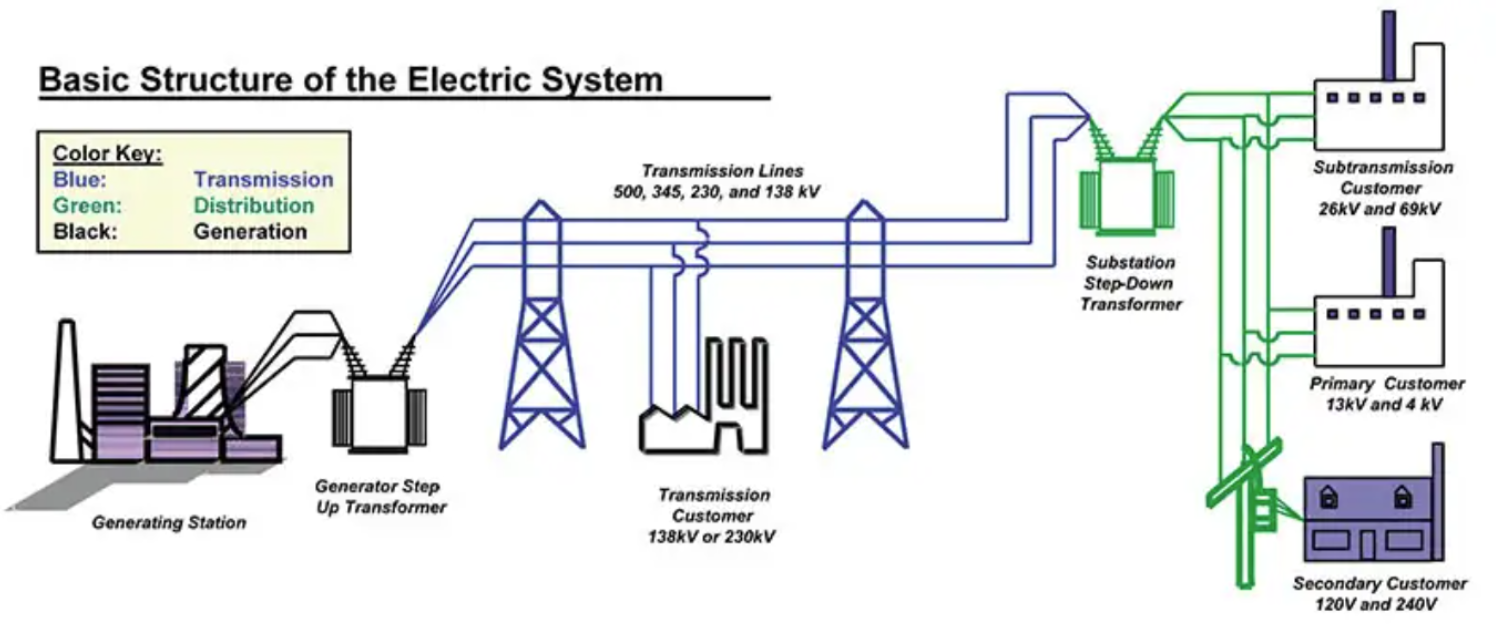
\includegraphics[scale=0.365]{graphic/basic-structure-of-the-bes.png}}
\caption{A conceptual illustration of the Bulk Electric System} 
\label{fig:BES_1}
\end{figure}

It is important to note that serving these various functions to provide electricity generates enormous amounts of data on an hourly basis. This data is widely diverse in terms of sourcing, formatting, usage, sensitivity, and volume. It is the data assets generated by the operation of the BES that serve as the focus of this dissertation, specifically in the data generated by \textit{electricity markets}.
\section{An Introduction to Electricity Markets}

A basic understanding of economics includes the concepts of supply and demand. Supply indicates that a seller has a good (usually a commodity \footnote{Commodities refer to the raw materials that are involved with manufacturing products. For example, crude oil is a commodity that is refined into kerosene, diesel, or gasoline.}
or product). When a consumer wishes to purchase that supply, it is referred to as a demand. The sale of supply results in the formation of a market. As stated above, this paper focuses on organized markets.  A large portion of the BES includes centrally organized electricity markets. Electricity markets are of great importance to all stakeholders involved in the BES; they allow energy to be economically generated for consumers.

\begin{figure}[ht]
\centering
\fbox{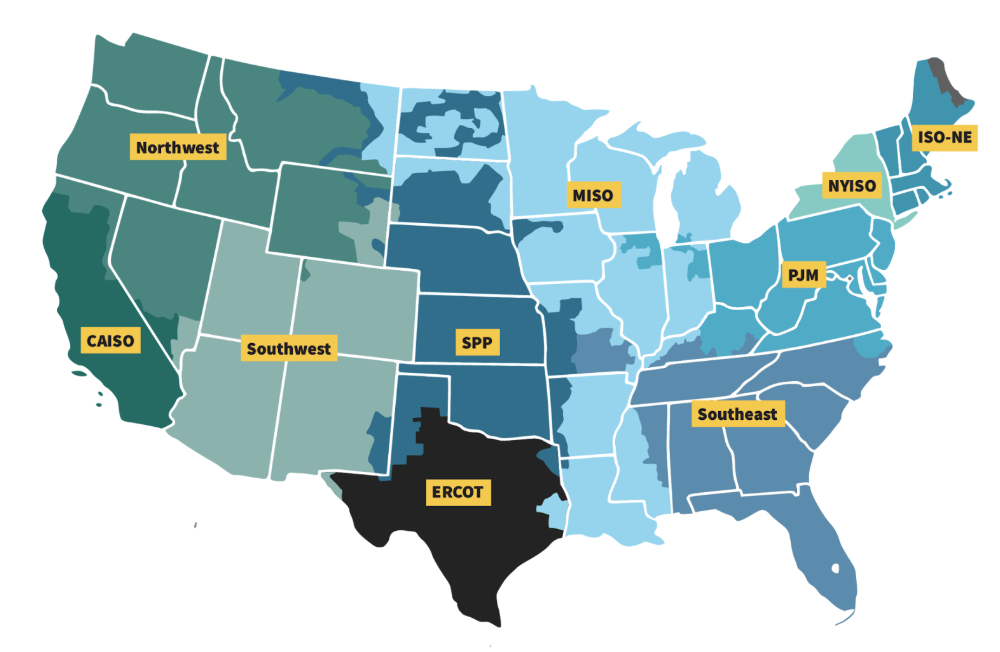
\includegraphics[scale=0.45]{graphic/us-grid-map.png}}
\caption{FERC Jurisdictional Market Territories}
\label{fig:gridmap}
\end{figure}

Figure \ref{fig:gridmap} \cite{ferc2} displays, at a high level, how the US energy grid is divided into different territories. These territories are typically governed by FERC, with the exception of Texas. ERCOT, the electric system operator for Texas, is not within the jurisdiction of FERC. The Public Utility Commission of Texas, instead, has oversight of the ERCOT market territory.

\subsection{Grid Operational Entities}
Electricity markets are operated by a small number of operational entities \footnote{"Grid Operational Entities", as referred to in this chapter, are not limited to the 2 categories listed. They also include Transmission Owners and Operators (TO / TOP), Regional Entities (RE), Balancing Authorities (BA), Reliability Coordinators (RC), and Federal Power Agencies. Oftentimes, an RTO or ISO will also support one or more of these functions (SPP, for example, hosts operational desks for performing reliability coordination).}
within North America. These entities fall under the jurisdiction of FERC, as indicated by Figure \ref{fig:gridmap}. The prominent entities that are impacted by market monitoring include Independent System Operators (ISO) and Regional Transmission Organizations (RTO). These entities are filed as non-profit businesses and typically perform similar functions. FERC Orders 888 and 889 initiated the formalized incorporation of an ISO, while FERC Order 2000 set forth the criteria that differentiates an ISO from an RTO.

\subsubsection{Independent System Operator (ISO)}

ISOs are organizations that manage power generation and transmission across the bulk electric system. They operate in an advisory capacity for generation owners (public and investor owned utilities, as well as independent power producers) and transmission owners and operators to effectively generate and trade power in an energy market. A common, helpful analogy that describes the function of an ISO is an air-traffic controller.

Air-traffic controllers merely monitor and route airplane traffic across the airspace over the United States. They own neither physical airplanes nor airlines, and function only as advisors to ensure safe passage of both private and commercial airplanes. ISOs work in a similar fashion. The ISO over the California energy market territory (CAISO) owns none of the transmission infrastructure across which electric power is shipped. However, CAISO manages the flow of energy across this system, and sends regular dispatch instructions to the generators that inject power into the BES.

\subsubsection{Regional Transmission Organization (RTO)}

According to the \textit{Energy KnowledgeBase} product maintained by Enerdynamics (an educational entity in the energy space), RTOs are categorized by a group of four core characteristics (and an additional seven broad operational functions). %CITATION% goes here...  item number 3 from original bibliography
The following lists identify these characteristics and functions that separate ISOs and RTOs. Although similar in nature; in fact, they are regulated by the same entities and have many of the same requirements under current law. It is important to note, however, that ISOs also operate energy markets and are subject to the same market monitoring requirements as RTOs. \\


\noindent Core characteristics of an RTO include:
\begin{enumerate}
    \item{Independent operation and authority from the market participants that join the RTO}
    \item{Maintain a "regional configuration"}
    \item{Maintain "operational authority for all transmission facilities under RTO control"}
    \item{Maintain short-term reliability of their footprint}
\end{enumerate}


\noindent Operational functions of an RTO include:
\begin{enumerate}
\item{Energy market design and “tariff administration”}
\item{Management of transmission capacity (FTR)}
\item{Management of flow on the transmission system}
\item{Support for ancillary services (AS)}
\item{Management of transmission capacity and capability, including imports and exports of power}
\item{Engineering support for planning the future state of the gid}
\item{Coordination between control boundaries}
\item{Market Monitoring}

\end{enumerate}

\subsection{Types of Markets}

Electricity markets are designed to serve one of several purposes. ISOs typically deploy and operate these different market designs, in concert, as a \textit{marketplace} \cite{ferc2}. Southwest Power Pool's (SPP) Integrated Marketplace is such an example of this. To understand the scope of market monitoring activities, it is important to understand the main energy market designs that exist today. Arguably, there are five main types of electric energy market designs; each design may be deployed with possible variations on their theme (a marketplace that does not operate the function of a capacity market is one such example). Reference Table \ref{tab:mktdesign} for information on prevailing design types.

\begin{table}[ht]
    \centering
    \renewcommand{\arraystretch}{1.2} % Adjust row height
    \begin{tabular}{|p{4.5cm}|p{11cm}|}  % Set fixed column widths
        \hline
        \textbf{Market Type} & \textbf{Purpose} \\ 
        \hline
        Capacity & Allows a load to purchase an agreement of firm capacity for service in the future- usually on the scale of months to years in the future. \\ 
        \hline
        Day-Ahead (DA) & Allows buyers and sellers to secure positions a day before the market sells energy to be consumed (operating day). This aids in realistic price formation. \\ 
        \hline
        Real-Time (RT) & Allows for adjustments between the DA market (what was expected on the day prior) and the system conditions that happen on the operating day. \\ 
        \hline
        Ancillary Services (AS) & Allows other providers to sell products that support grid reliability. For example, the ability of a generator to quickly “ramp up” to a certain production requirement is such a product sold in an AS market. \\
        \hline
        Transmission Congestion Rights & Allows participants to hedge against congestion on the transmission system (adequate power can be produced in an area, but there may be difficulties in transmitting it to where it is consumed). \\
        \hline
    \end{tabular}
    \caption{Prevailing Electricity Market Designs}
    \label{tab:mktdesign}
\end{table}

\subsection{Market Complexity}

The BES is a physical system upon which we superimpose a conceptual, economic market. This dichotomy is part of what makes the energy market so complex to both understand and govern with the data that it generates. Physical machines require continuous diagnostics to ensure that they are operating 1) effectively and 2) within adequate maintenance tolerances. The BES is no different.

Thermal generators that produce electricity are monitored for metrics including: wattage output, fuel consumption, greenhouse gas emissions. High-voltage transmission lines are monitored for temperature (heat is generated via electricity loss across conductors) and short-circuit events. Substations are monitored for transformer faults, tap configurations, and other mechanical system measurements. Each of these values is typically transmitted in a time-series format, resulting in constant streams of monitoring data. These time series data streams are typically parsed into \textit{market intervals} that constitute "units of work" for market activity. Much of the analysis performed on wholesale electricity markets utilizes data secured from market intervals. Depending on the type of market that is under observation, an interval may range from a span of several seconds (dispatch instructions) to "between five and fifteen minutes" \cite{ferc1} (calculation of real-time market prices). 

These diagnostic data are only a fraction of the data that are used in the operation of the BES, and much of it feeds into market systems \footnote{While market systems are composed of many different products, they are generally referred to as a \textit{market clearing engine}.} to calculate a realistic price of power at different locations throughout a market territory.

\subsection{Market Settlements}

Another subject area of the BES that generates complex and voluminous data includes a collection of processes that perform \textit{market settlements}. In SPP's Integrated Marketplace, the Marketplace Protocols set forth an extensive settlement plan that determines how charges and credits are calculated and assigned to market participants. These settlement instructions also take into account events where the market must be "repriced", or re-settled due to external factors that occur during the operation of a market- such as equipment outages, data communication errors \footnote{Data elements used to monitor and dispatch generation in the BES are collected and shared in the form of \textit{SCADA} (Supervisory Control and Data Acquisition) \cite{scada1}.}, or extreme weather events.

Market settlements also generate enormous data volumes due to another necessary function: \textit{shadow calculations}. Shadow calculations \footnote{Shadow accounting involves the process of maintaining a separate system (in addition to a production accounting system) to track transactions and ensure that accounts are appropriately balanced. \cite{shadow-acct}} 
are necessary in energy markets due to both the regulatory landscape and the fact that market participants leverage millions of dollars in capital during energy production and sale.

\section{What is Market Monitoring?}

Market monitoring is a discipline that sits at the intersection of two major knowledge domains: \textit{forensics} and \textit{economics}. As such, it takes a scientific approach to testing and analyzing transactions that occur within a marketplace. According to a report published by the United States Energy Association (USEA), Market Monitoring is a necessary component of markets "to ensure that market(s) participants cannot exercise market power, collude or engage in any other behavior that could give them a great market share, or higher profits" \cite{imm-usea}. This appointment places the authority to request and analyze records generated by the operation of electricity markets into the hands of MMUs.

Market monitors will generally screen for MP behavior that matches the following criteria:

\begin{itemize}
    \item{Exercised (or attempted to exercise) positions of market power}
    \item{Market gaming through oversights in current market protocols or policy (usually outlined in a governing document, known as a Tariff}
    \item{Committed cases of market manipulation through acts of collusion, cross-product manipulation, malevolent influence on price formation, or untoward manipulation schemes (economic withholding, uneconomic production, wash trades, "pump and dump" schemes, etc.}
\end{itemize}


\subsection{The Fall of Enron Corporation}

Enron Corporation, a former American-based commodities and energy broker, is a well-known case study in American corporate governance (or, rather, lack thereof). The fall of Enron (first signaled in late 2000) uncovered deep, systemic problems of fraud and deceptive business practices that directly influenced both the market monitoring and IQ disciplines. If taken at face value- Enron appeared to be a stable and innovative company. At the turn of the century, Enron's books reflected an ownership of \$60 billion in assets. This included an internet-based energy trading desk ("Enron Online") that cleared \$2.5 billion in \textit{daily} energy transactions \cite{enron-financials}. In reality, Enron management operated under a culture of willful non-compliance, including (but not limited to):

\begin{itemize}
    \item{Withholding practices that caused enormous electricity prices in the California power market- ultimately bankrupting Pacific Gas and Electric (PG\&E).}
    \item{Artificial energy shortages causing regular blackouts \footnote{A blackout (an event where power cannot be served) is a breakdown of a portion of grid infrastructure, caused by "an imbalance between power generation and power consumption" \cite{nerc1}.}
    in California- a serious threat to both energy reliability and human welfare.}
    \item{Accounting fraud (enabled by a creative use of “mark-to-market” based accounting) which allowed Enron to report expected revenues before they were realized.}
\end{itemize}

Enron’s activities constitute behavior known as \textit{market manipulation}; a form of conduct that attempts to wilfully circumvent established market rules in pursuit of (usually) large profits. This behavior often is a result of an abuse of \textit{market power}, where a participant or operator knowingly takes positions to inflate the price of electricity at a location in a market territory. Their usage of market manipulation, especially in California, was a signal to federal regulators that, at the time, there was not enough oversight in the operation of electricity markets. As a result, the United States Congress passed the Energy Policy Act of 2005 to introduce more stringent regulation over the energy industry.

Enron’s downfall resulted in a near-complete devaluation of their stock \footnote{As Enron entered into legal proceedings, their stock fell to under \$1 per share (from a peak as high as \$90 per share in mid-2000) \cite{enron-stock-chart}. }
, the dismantling of Arthur Andersen, (the auditor assigned to ensure that Enron was operating within the confines of financial reporting law), and a slew of legislation \footnote{18 CFR § 1c.2 (Prohibition of Electric Energy Market Manipulation) is an example of legislation that places monitoring authority in the hands of MMUs \cite{ecfr1}.} 
serving as the impetus for energy market monitoring in the United States. Additionally, Enron’s scandal was a significant contributor to the passing of the Sarbanes-Oxley (SOX) Act of 2002, imposing strict and detailed requirements on data that is used as input for financial reporting. As a result, SOX became another driving force in the implementation of Information Quality as both an academic discipline and as a business function.

\subsection{Skills of a Market Monitor}

Market monitors are one of several groups that function as "unsung heroes" in electricity markets (and within the larger context of the North American bulk electric system). The work that they perform on a routine basis helps to ensure a reliable and economically sound marketplace for buying and selling energy and energy-adjacent ancillary services. Market monitoring units are typically staffed with analysts from a wide variety of both technical and non-technical backgrounds. These include: data analysts, statisticians, economists, accountants, technical writers, and other corporate staff dedicated to investigating events that occur in their jurisdictional markets.

\begin{figure}[h]
\centering
\fbox{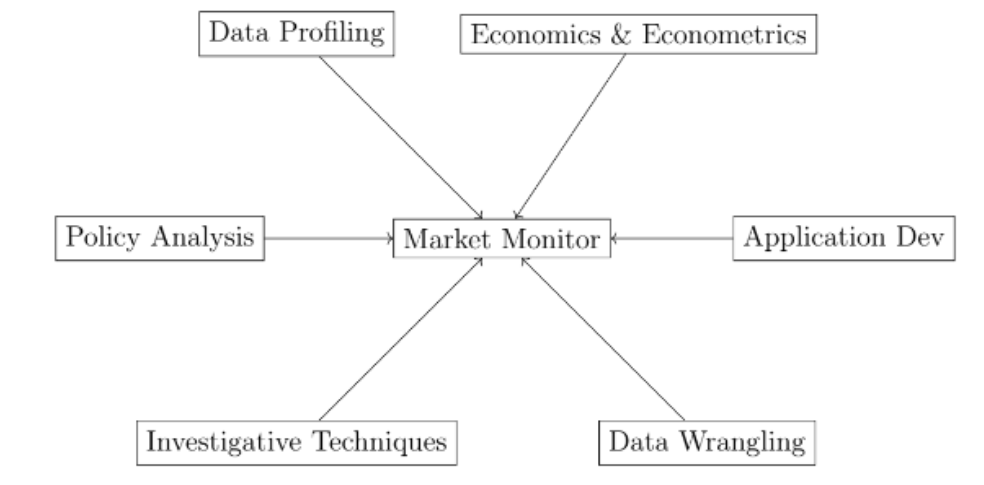
\includegraphics[scale=0.5]{graphic/mkt-monitoring-skill-sets.png}}
\caption{Diverse skill sets of a Market Monitor}
\label{fig:skillset}
\end{figure}

Figure \ref{fig:skillset} illustrates a cross-section of several of the skill sets that market monitoring analysts might possess, based on the researcher's experience of working as a market monitor within Southwest Power Pool's (SPP) MMU. As one may imagine, it can be difficult to find an individual contributor that possesses an all-encompassing understanding of each of these knowledge areas.

\subsection{Landscape of Market Monitoring}

Market monitors have a wide breadth of responsibilities that must be covered by their individual skill sets. Routine market surveillance is a continuous process that must evolve with the behaviors and trading patterns of market participants. As such, market monitors have to observe and investigate market bids and offers made each operating day, analyze generator behavior to identify erratic response to dispatch commands, ensure that participants are not covertly colluding or engaging in price fixing \footnote{Energy market prices are typically set on a marginal, spatial basis (representing the cost of injecting another MW of energy, at a location, in a market territory) \cite{lmpfaq}.}, and ensure that RTOs and ISOs are acting within the rules defined by their FERC-approved Tariff
\footnote{A Tariff is a governing document that outlines the rules for operating (and participating in) an energy market.} documents. 

\subsubsection{Market Monitoring Firms}

The current groups involved with electricity market monitoring (both in North America and internationally\footnote{The US Energy Association (USEA) published a report outlining international, independent market monitoring groups. Many of the international groups on this list come from that report (see References).}) include the following organizations compiled in Table \ref{tab:mmu-roster}. This list is not intended to be exhaustive, as other nations \footnote{See the list of Industry Acronyms for definitions of these regions} in APAC and EMEA may not be reflected here.

\begin{table}[ht]
    \centering
    \begin{tabular}{|p{6cm}|p{5cm}|p{2cm}|}
        \hline
        \textbf{Name of Firm} & \textbf{Market Affiliation} & \textbf{Country} \\
        \hline
        Federal Energy Regulatory Commission (FERC) & Jurisdictional oversight for all US-based energy markets & USA \\
        \hline
        SPP MMU & Southwest Power Pool (Internal) & USA  \\
        \hline
        Potomac Economics & MISO, ERCOT, NYISO, ISO-NE (External) & USA \\
        \hline
        ISO-NE IMM & ISO-NE (Internal) & USA \\
        \hline
        CAISO MMU & California ISO (Internal) & USA \\
        \hline
        Monitoring Analytics & Pennsylvania, New Jersey, Maryland Interconnect (PJM) & USA \\
        \hline
        Market Surveillance Administrator & Alberta & Canada \\
        \hline
        Independent Electricity System Operator (IESO) & Ontario & Canada \\
        \hline
        Canada Energy Regulator & Jurisdictional oversight for all Canadian energy markets & Canada \\
        \hline
        Superintendencia de Electricidad y Combustibles & - & Chile \\
        \hline
        Agencia Nacional de Energia Electricia & - & Brazil \\
        \hline
        Ente Regulador de la Electricidad & - & Argentina \\
        \hline
        Superintendencia de Electricidad & - & Bolivia \\
        \hline
        Regulation on Wholesale Energy Market Integrity and Transparency (REMIT) & European Union Agency for the Cooperation of Energy Regulators & Europe \\
        \hline
        AER & Australian Energy Regulator & Australia \\
        \hline
        NZEA & New Zealand Electricity Authority & New Zealand \\
        \hline
    \end{tabular}
    \caption{A Roster of Groups with Market Monitoring Authority}
    \label{tab:mmu-roster}
\end{table}

\section{Conducting Information Quality Research in Market Monitoring}

The case-study of Enron Corporation sets both a unique and compelling stage for the role that Information Quality and Information Science-based research can play in improving the business impact of an independent market monitor. Included amidst Enron Corporation’s numerous failures of governance is a lack of access and understanding of the complex data generated by the energy industry. The operation of such a large system and marketplace can lead to many siloed data stores, undocumented schemas, and a slew of other IQ-based problems that can also be seen in market monitoring.

Furthermore, the cross-section of skills that market monitors must possess (to effectively perform their job functions) also underscores the importance that data literacy and data quality improvement hold in the market monitoring domain. An architecture solution, proposed as part of the deliverables of this dissertation, is paramount to designing a system to aid market monitoring staff in their work.

\subsection{Subject Matter Expert (SME) Discussions}

The potential use of this dissertation is driven, in part, by the opinions of subject matter experts in the field of electric energy. In support of this research, I have consulted multiple members in different sectors of the industry, including 2 professionals in enterprise asset management, and a separate discussion with a staff member in energy regulation. One such staff member, Dr. Kennedy Oyoo, performed information systems research in a different sector of the energy grid- “power and utilities”- focusing on the distribution of electricity to end users.

Energy utilities struggle with a similar issue to those faced by market monitors- siloed data exists in different systems, and can exist with vastly different data quality scores (in terms of completeness, accuracy, etc.) Dr. Oyoo’s research found that a key step- data validation- was missing from the ETL processes of an energy utility. Part of the research completed in his project resulted in an information template-based prototype system that cleansed and validated utility data according to automated assertion rules. Such a methodology has potential impacts for the market monitoring discipline, and can have an influence on the resulting system architecture of this dissertation (particularly in utilizing a system of templates to fetch market data).

%%%%%%%%%%%%%%%%%%%%%%%%%%%%%%%%%%%%%%%%%%%%%%%%%%%
%
%  New template code for TAMU Theses and Dissertations starting Spring 2021.  
%
%
%  Author: Thesis Office
%  
%  Last Updated: 1/13/2021
%
%%%%%%%%%%%%%%%%%%%%%%%%%%%%%%%%%%%%%%%%%%%%%%%%%%%

%%%%%%%%%%%%%%%%%%%%%%%%%%%%%%%%%%%%%%%%%%%%%%%%%%%%%%%%%%%%%%%%%%%%%%%
%%%                           SECTION II (IX - this is a section II re-write)
%%%%%%%%%%%%%%%%%%%%%%%%%%%%%%%%%%%%%%%%%%%%%%%%%%%%%%%%%%%%%%%%%%%%%%


\chapter{\MakeUppercase{Literature Review}}
\label{cha:literature-review}

A review of the literature surrounding information quality research within market monitoring units signals that there is room for improvement in how value is generated from information assets. This gap is highlighted by several major issues (introduced in Chapter \ref{cha:Introduction} and discussed in this literature review), including:

\begin{enumerate}
    \item {Development of technology surrounding domain-specific language engineering}
    \item {An aging workforce in the electric utilities industry that is reaching the tipping point for replacement}
    \item {A lack of existing research on data and information quality within the market monitoring sphere}
    \item {A disruption of traditional energy market design due to advances in technology and the energy regulatory landscape}
\end{enumerate}

\noindent These issues represent a unique opportunity to obtain important value from the data assets both generated and used by professionals in the market monitoring sphere. The researcher will discuss each of these issues in the context of relevant literature\footnote{Appendix \ref{appendix:B} contains a listing of different search phrases used for locating relevant research discussed in this chapter.},
and then introduce possible sources of data that enable the development of a domain-specific language for market monitors.% ecg0122 - commenting this out since I rearranged these sections based on Dr. Berleant's recommendation indicate how this design science project has the potential to improve these issues within market monitoring.

\section{An Aging Workforce}

Many technical industries are experiencing the problem of an aging workforce; trained professionals are reaching retirement age at a rate faster than that of replacement. A 2006 study showed that the largest staff segment, of a surveyed group of energy professionals, is at (or beyond) retirement age. This same study cited "retirements, restructuring, and technology changes" as being the primary drivers of staff leaving the energy profession \cite{raysnyder}. Given the age of this study, many industries are currently going through a period of training new career professionals. Such a problem impacts market monitoring as well. 

MMUs (as previously discussed) were cemented into operation by the US federal government, not long before that same 2006 study. An energy research lab at UC Berkeley shows that staffing across market monitoring groups is relatively low compared to other organizations in the industry. According to Goldman, Lesieutre, and Bartholomew, all operational market monitoring groups in the US had fewer than 20 FTEs (each) in employ by 2004 \cite{goldman}.

While these numbers appear low in comparison to other organizations with energy industry staff\footnote{As of Q1 2025, Southwest Power Pool employs over 800 FTEs (including their internal market monitoring staff).}, this study declares that budgets and headcount (at that time) increased significantly for market monitoring work. As such, this shows a trend of growing demand for market monitoring staff in a workforce that, holistically, employs many individuals on (or beyond) the horizon of retirement. One claim to helping combat this "brain drain" problem is a technology framework that "facilitates knowledge retention" \cite{raysnyder}, including systems (supported by an IT organization) that capture necessary process knowledge.

\subsection{The Importance of Institutional Knowledge}

Given that the energy industry faces career professionals heading into retirement, this research intends to use a domain-specific language-based system to help preserve the institutional knowledge that is lost when market monitors retire (or even simply change positions). As employees make career transitions, the institutional knowledge that they built often leaves with them. In market monitoring, this problem is amplified due to two salient facts: 1) the number of individuals that work in market monitoring is small compared to the rest of the energy and utilities industries, and 2) market monitors often specialize in regards to analysis or policy work. Individuals who primarily work in market surveillance may never directly work in policy development (or vice-versa).

In a personal anecdote, this "brain drain" problem has been seen within the SPP MMU. Several long-term employees have exited the MMU in pursuit of other roles, only to leave undocumented code behind them that others must support. This code exists in the form of SQL queries and/or SAS scripts that contain embedded business rules (as they were understood by these employees). Deciphering and supporting this code becomes a burden for others that inherit the work of these departed employees.

A 2016 publication \textit{Knowledge Management in Esoteric Management} summarizes this issue well: "...knowledge sharing should be encouraged by placing employees working together closely to create pooled expertise..." \cite{knowledge-management-in-esoteric-management}. When employees share knowledge, they can keep important information from being destroyed when key individuals leave a department. One of the goals for the system that this dissertation designs is to foster knowledge sharing amongst employees.

\subsection{Application to Market Monitoring Research}

%As the previously discussed examples exhibit, 

Domain-specific programming languages (DSLs) are powerful interfaces that enable subject-matter experts (SME), in any particular domain of expertise, to perform tasks similar to a proper software developer that builds applications in general-purpose languages (GPL). A well-defined DSL can save many hours of development time for specific groups that have IT oriented needs. DSLs also have the ability to lower the "barriers to entry" for SMEs that wish to write applications to handle work within their purview. With support from a DSL, a software engineer does not need to be deeply involved in business rules to understand how to develop an application (a common issue in the energy industry). Likewise, SMEs do not need to heavily codify their business rules into software requirements for an application to be developed when utilizing a domain-specific language.

Following the theme of how DSLs are able to abstract away complexity of big data processing tasks, this research aims to bring such a tool set to bear on tasks performed in energy market monitoring. Commands embedded into a domain-specific language have the potential to speed up many repetitive tasks in the market monitoring domain, especially regarding the generation of report and stakeholder presentations.

\section{An Analysis of Domain-Specific Languages}

Consider programming languages on a spectrum from general purpose languages (GPLs) at one end to domain-specific languages (DSLs) on the opposite end \cite{tomaz-dsl}.\footnote{Kosar, Tomaz, et al. indicate the "schism" between the two languages by discussing that "GPLs tend to be general, resulting in
poor support for domain-specific notation \cite{tomaz-dsl}."}
DSLs are languages that are limited in purpose, scope, and grammar. Rather than supporting a programming language that can be utilized for constructing almost anything (as GPLs do), DSLs are created to solve issues within a single problem domain.

\begin{table}[ht]
    \centering
        \begin{tabular}{|p{6cm}|p{4cm}|p{4cm}|p{2cm}|}
        \hline
        %https://aws.amazon.com/what-is/sql/
        \textbf{Language} & \textbf{Supporting \newline Enterprise} & \textbf{Problem Domain} & \textbf{Paradigm} \\
        \hline
        Structured Query Language (SQL) & Various & Data Retrieval & Declarative \\
        \hline
        %https://developer.hashicorp.com/terraform/intro
        Terraform / HCL & Hashicorp & Cloud Infrastructure \newline Deployment & Declarative \\
        \hline
        %https://pig.apache.org 
        Apache Pig ("Pig Latin") & Yahoo / Apache \newline Software Foundation & Data Retrieval \newline \& Processing & Declarative \\
        \hline
        %https://dev.to/jpmcb/awk-a-beginners-guide-for-humans-3l25
        awk & Bell Labs (originally) & Text Processing & Procedural \\
        \hline
        \end{tabular}
    \caption{Selection of Well-Known Domain-Specific Languages}
    \label{tab:well-known-dsl}
\end{table}

\textit{Structured Query Language (SQL)} \cite{dsl-aws} is one such example of a DSL. SQL queries are designed to retrieve data from databases for extraction, reference, and analysis. SQL dialects have been designed to interface across a broad range of database management systems (for example: PL/SQL for Oracle or T-SQL for Microsoft SQL Server databases).

\textit{Terraform (HCL)} \cite{dsl-terraform}, a product of Hashicorp Corporation, is yet another example of a domain-specific language that is prevalent among cloud-based companies. Terraform is known as an "infrastructure-as-code" language, used to interact with numerous cloud platform providers (e.g. Amazon Web Services) to quickly deploy, scale, and spin-down cloud resources. Instead of requiring an engineer to use a console environment to configure cloud resources, that same engineer can write a set of scripts that will precisely configure and deploy all of their desired infrastructure at once.

\textit{Apache Pig} \cite{dsl-pig-latin} (and its associated programming language \textit{"Pig Latin"}) is also a DSL. Like SQL, it is a declarative language used for data retrieval and data processing. Developers at Yahoo created Pig as a way to abstract some of the complexity of SQL away from analysts who were working with large datasets. With fewer lines of code, an analyst could use Pig to parse and load a dataset into memory, perform processing tasks, and format and report the results. This was specifically useful to analysts processing large datasets because Pig was designed to take advantage of the high-performance computing facilities of Hadoop.

Yet another powerful example of DSLs can be seen in the ubiquitous Unix program: \textit{awk} \cite{dsl-awk}. Originally created by Unix developers Aho, Weinberger and Kerninghan\footnote{The name "awk" is an acronym formed from the first letters of the developer's last names.}, awk is a scripting language designed to process textual data--- one line at a time. The power of this systems allows individuals to write expressions that are simple to understand, efficient, and portable across different Linux implementations. Countless developers (including the author of this dissertation) have made use of awk's utilities to process and format data in a headless environment.

Each of the languages represented in this review are, on their own, infeasible for writing general purpose applications. SQL, for example, should not be used to write a desktop program. They were, instead, each created to solve specific issues within their respective problem domains. Likewise, Terraform cannot be used to create web applications or develop billing software. One of the "upsides" of these languages are that they can quickly handle tasks within a specific problem domain.

\subsection{DSL Variations}

Each of the language examples provided here share a common characteristic in that they are external DSLs. They are interpreted and executed by a runtime program. This trait of DSLs separates them from another subset of domain-specific languages: internal DSLs. These are embedded langauges (sometimes referred to as fluent interfaces) that rely on a (usually) general-purpose language to parse their individual syntactic structures and execute logic. These DSL features are sometimes referred to as \textit{syntactic sugar} \cite{syntactic-sugar}, implying that they make the experience of developing solutions in them "sweeter" than without them.

Another common characteristic of DSLs lies in the fact that they are often text-based programming environments. As discussed later in this literature review, graphical domain-specific languages also exist. These are usually seen in the form of either enterprise extract-transform-load (ETL) applications or language workbenches. Jetbrains MPS is a prominent example of the power of graphical DSL representations. Business users are usually positioned to take advantage of these product offerings because they pose abstract interfaces (environments that allow users to graphically model \textit{what they want} instead of having to explicitly write source code in a general purpose language). With basic instruction, users can string together components that construct repeatable workflows without requiring them to possess deep programming knowledge.

\section{Extant Domain-Specific Language Use Cases in the Energy Sector}

The literature uncovered in this review supports the claim that DSLs can achieve high efficacy in financial contexts. Krasts, Kleins, and Teilans (2012) illustrates how domain-specific languages have been used in modeling the complex dynamics of financial settlements systems. Financial settlements often encounter system error cases during the settlement of a market. Using a DSL for modeling tasks, in these scenarios, appears to help developers and business users clearly visualize complex systems logic \cite{krasts}.

The literature, even more interestingly, shows that DSLs have been deployed in other areas of the energy sector, as identified by Sobernig, Strembeck, and Beck \cite{beck} in \textit{Developing a Domain Specific Language for Scheduling in the European Energy Sector}. While this paper sets precedent for the use of DSLs in the energy industry, it presents an even larger gap that this dissertation addresses. Beck's study explores employing a DSL to assist in tagging and scheduling energy interchange (which is an operational concern that only encompasses a single component of market monitoring). Additionally, and far more importantly, the implementation of their DSL was constrained to a specific market interconnection in Europe, which is significantly less complex than the transmission and congestion\footnote{Current issues in North America show large pockets of stranded load, which have significant economic (and, by extension, reliability) implications. Congestion on the BES constitutes a market (Financial Transmission Rights - FTR) that settles for billions of dollars. This is all due to the fact that monies have to be paid to rights holders for transmitting energy across a congested transmission infrastructure.}
issues that are seen throughout the North American Bulk Electric System. Market monitoring, while interested in aspects of transmission scheduling, encompasses a much broader scope of analytics in the energy sector. 

\section{The Data Domain in Market Monitoring}

The data domain for market monitoring entities is a large ecosystem. It is common for monitoring analysts to synthesize information both from internal and external data sources. This type of ecosystem can quickly become a \textit{data swamp}\footnote{Atlan, a leading data governance company, classifies a data swamp as a repository that possesses: poor quality, undocumented code and data schemas, and leads to situations where users must "...spend considerable time on tasks such as data discovery, cleaning, integration, and management" \cite{atlan-data-swamp}.} without careful attention to business rules and the possession of institutional knowledge for how processes are executed on market information.

FERC Order 760, a key piece of legislation that directly relates to this dissertation, is one such example of how market data is sourced and utilized by analysts. It dictates several key categories of data that RTO/ISO organizations must regularly provide to the Commission. Such data includes \cite{daignault}:

\begin{enumerate}
    \item{Supply offers and demand bids for energy and ancillary services}
    \item{Virtual\footnote{A "virtual" transaction (as defined by Southwest Power Pool's glossary of terms) is a transaction for purchasing (bid) or selling (offer) energy "at a specified price, settlement location, and period of time ... that is not associated with a physical load" \cite{spp-virtual-bid-offer}.} offers and bids}
    \item{Energy/ancillary service awards}
    \item{Capacity market offers, designations, and prices}
    \item{Resource (electricity generation) output}
    \item{Marginal cost estimates}
    \item{Day-ahead market (DA) shift factors\footnote{A \textit{shift factor} is a percentage based value that determines how much energy a transmission line will receive when a generator injects energy into the transmission grid \cite{epe-shift-factor}.}}
    \item{Financial Transmission Right (FTR) data}
    \item{Bilateral Contracts}
    \item{Interchange transactions (otherwise known as "scheduling and tagging")}
\end{enumerate}

Understanding how to source and use this information impacts the accuracy of market monitoring analysis and enables FERC to accurately assess and penalize instances of market manipulation. Defined by the industry terms "ex-ante" and "ex-post", assessments of market performance, market power, and market manipulation can be carried out prior to an event, or "after the fact"- when a market event has already occurred \cite{green-neuhoff-newberry}.

\subsection{Public Data Systems for Wholesale Energy Markets}

In a similar manner to how market operators provide regular data to FERC, RTOs and ISOs also regularly publish data that allows the general public\footnote{See Appendix \ref{appendix:D} for a list of hyperlinks to view more information on these public sources of energy market data.} a view into the operation and settlement of these markets. Table \ref{tab:public-data-repos} lists the existing systems that this research can utilize for test data. Much of the data contained in these systems match the data requirements for FERC Order 760 (though some identifiers may be omitted or obfuscated to preserve confidentiality).  

The researcher intends to source data assets that model market conditions (especially for price formation) from these systems, and use such data for demonstrating the abilities of the prototype system, including: 1) visualization generation, 2) report creation, and 3) shadow calculations. The data assets that may be necessary to produce the demonstration deliverables include public records such as generator names and parameters, generation outages, transmission line data, and component data used to calculate marginal prices (energy, loss, and congestion factors). 

\begin{table}[H]
    \centering
        \begin{tabular}{|p{6cm}|p{6cm}|}
        \hline
        \textbf{Publishing Entity} & \textbf{Data Repository Name} \\
        \hline
        PJM Corporation & Data Miner 2 \\
        \hline
        Monitoring Analytics & Member Information Reporting \newline Application (MIRA) \\
        \hline
        Electric Reliability Council \newline of Texas (ERCOT) & Market Data Transparency Service \\
        \hline
        California Independent System \newline Operator (CAISO) & OASIS \& Data Library \\
        \hline
        Midcontinent Independent System \newline Operator (MISO) & MISO Data Exchange \\
        \hline
        Southwest Power Pool (SPP) & Public Data Portal \\
        \hline
        New York Independent System \newline Operator (NYISO) & Operational Data Portal \\
        \hline
        Independent System Operator of \newline New England (ISO-NE) & ISO Express \\
        \hline
        US Energy Information \newline Administration (EIA) & Wholesale Energy Market Reports \\
        \hline
        \end{tabular}
    \caption{Public Energy Market Data Systems}
    \label{tab:public-data-repos}
\end{table}

\pagebreak

%\begin{figure}[H]
%\centering
%\fbox{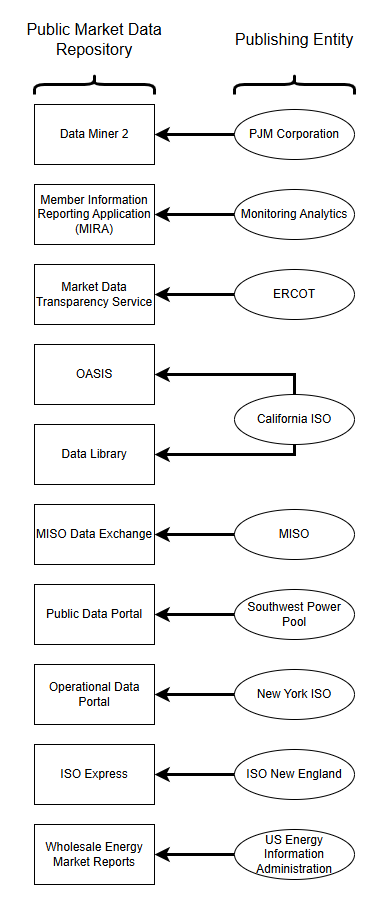
\includegraphics[scale=0.85]{graphic/market-comps.png}}
%\caption{Public Market Data Sources}
%\label{fig:market-comps}
%\end{figure}

%\section{Design Science Methodology}
%
%The roadmap of this project is based on the Design Science Research Methodology (DSRM), a research process for developing new product artifacts. The researcher chose DSRM for this project because the main research objective is to design and develop a domain-specific language for market monitors to use in their analysis.

%Data and information quality problems exist today in the market monitoring body of knowledge that a DSL-based system can help address: 

%\begin{enumerate}
%    \item {Analysts in different teams that arrive at different values when trying to quantify metrics (market impact, for example)}
%    \item {Lack of robust metadata assets such as data dictionaries and well-defined data stewardship roles}
%    \item {Lack of a mature change management program for software (which, in turn, can impact report reproducibility) }
%    \item {A lack of full automation and meta-automation, causing analysts to spend time performing tedious ETL and archival tasks}
%\end{enumerate}

%Domain-specific languages are powerful models for allowing users to systematically solve problems within a specific domain. As was determined in this literature review, DSLs have only had limited exposure in electricity markets (and even less exposure in market monitoring). This discovered gap in existing research, complemented by the DQ and IQ issues stated in this review, serves as the inspiration for this project. Figure \ref{fig:dsrm} provides more detail on the planned use of design science within this project\footnote{See Appendix \ref{appendix:C} for a schedule of the milestones and expected completion timeline for this project.}.

%\begin{figure}[h]
%\centering
%\fbox{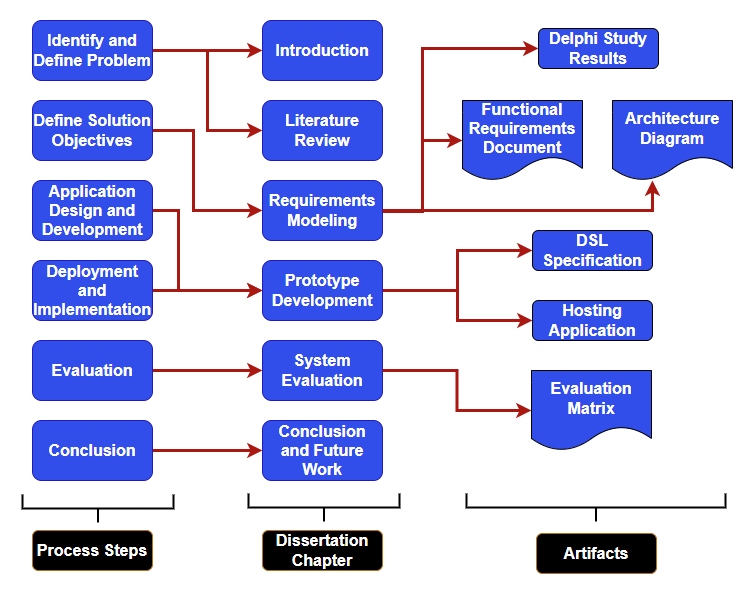
\includegraphics[scale=0.65]{graphic/dsrm_updated_20250819.png}}
%\caption{Design Science Research Methodology for this Dissertation}
%\label{fig:dsrm}
%\end{figure}

%\subsection{Proposed Investigation}

%In \textit{What Design Science Is Not (2008)}, Baskerville states that one view of design science is to be \textit{generative}. That is, design science leads to the generation of artifacts that then influence the formulation of a theory \cite{design-science-is-not}. This prospect of generativity seems to indicate that a design can be updated based upon empirical evidence. Due to this idea, the researcher chose to employ a Delphi study (as the methodology for gathering expert sentiment) to influence the design of the DSL prototype discussed in this dissertation. The following chapter discusses the setup, conduct, and results of a Delphi study employed in market monitoring. It then explains how the results of this study influenced the design and requirements document for the prototype system.

%Overall, the investigation methodology for this dissertation is composed of five (5) main components. These components include 1) a literature review, 2) a Delphi study to gather opinion and synthesize system requirements, 3) a system architecture design, 4) development of the prototype system (and associated tooling and documentation), and 5) an evaluation discussion to determine to what degree the resultant software honors the system requirements.

%\subsection{Limitations of this Research}

%The scope of work proposed in this dissertation is limited to the objectives outlined in the Proposed Investigation section. Specifically, it shall ultimately evaluate how well the developed prototype functions as a \textit{minimal viable product} (MVP) for energy market analysis.

%The proof-of-concept prototype discussed in this dissertation \textbf{is not intended to be a production-ready system}. It is also not expected to be used in a live scenario for market monitors to immediately put into service in support of decision making. The data ingested into the prototype will be based on realistic data scraped from public data systems shown in Appendix \ref{appendix:D}. The evaluation of this system will be based on a matrix (mapping back to the functional requirements document) that "scores" how well the functionality of the prototype supports the intended requirements.

%Further system optimization, bug fixes, scalability concerns, and use in live market monitoring scenarios are all currently considered "out of scope" for this dissertation and are reserved for future work. The author, however, may pursue future enhancements to this system as separate research endeavors.

%%%%%%%%%%%%%%%%%%%%%%%%%%%%%%%%%%%%%%%%%%%%%%%%%%%
%
%  New template code for TAMU Theses and Dissertations starting Spring 2021.  
%
%
%  Author: Thesis Office
%  
%  Last Updated: 1/13/2021
%
%%%%%%%%%%%%%%%%%%%%%%%%%%%%%%%%%%%%%%%%%%%%%%%%%%%

%%%%%%%%%%%%%%%%%%%%%%%%%%%%%%%%%%%%%%%%%%%%%%%%%%%%%%%%%%%%%%%%%%%%%%%
%%%                           SECTION III (This "chapter" is meant to be included in the proposal document only!)
%%%%%%%%%%%%%%%%%%%%%%%%%%%%%%%%%%%%%%%%%%%%%%%%%%%%%%%%%%%%%%%%%%%%%%


\chapter{\MakeUppercase{Proposal Methodology Plan}}
\label{cha:proposal-methodology}

Design science shall be used as the primary method of investigation in this dissertation due to its ability to derive insights from the development of new artifacts. However, design science itself is only a process that guides the investigation. To effectuate this process, the researcher has developed the following plan to build and evaluate a software system (powered by a domain-specific programming language) for potential use in the professional domain of energy market monitoring.

This plan includes the following details (illustrated by Figure \ref{fig:deliverable-plan}):

\begin{itemize}
    \item{A literature review to both introduce the research area and to establish relevance and novelty}
    \item{A Delphi-based study using a panel of experts (within market monitoring) to identify the current needs of these experts\footnote{The results of this panel shall serve as the basis for constructing a comprehensive software requirements document used during the development of this system.}, including:}
        \begin{itemize}
            \item{The current landscape of a market monitor's workflow}
            \item{Perspectives from the entire market monitoring community, including market monitors that work outside of the United States}
        \end{itemize}
    \item{A comprehensive data and system architecture plan for setting up and operating a DSL-enabled data analysis system}
    \item{Development of a prototype system to serve as a proof-of-concept for using a DSL in the context of market monitoring analysis}
    \item{Develop a \textit{traceability matrix} \cite{pm-traceability-matrix} that can serve as a method of evaluation, for this system, to ensure that the prototype serves the intended functional requirements}
    \item{A discussion of the performance of the system (as this also impacts the system's usability).}
\end{itemize}

\begin{figure}[ht]
\centering
\fbox{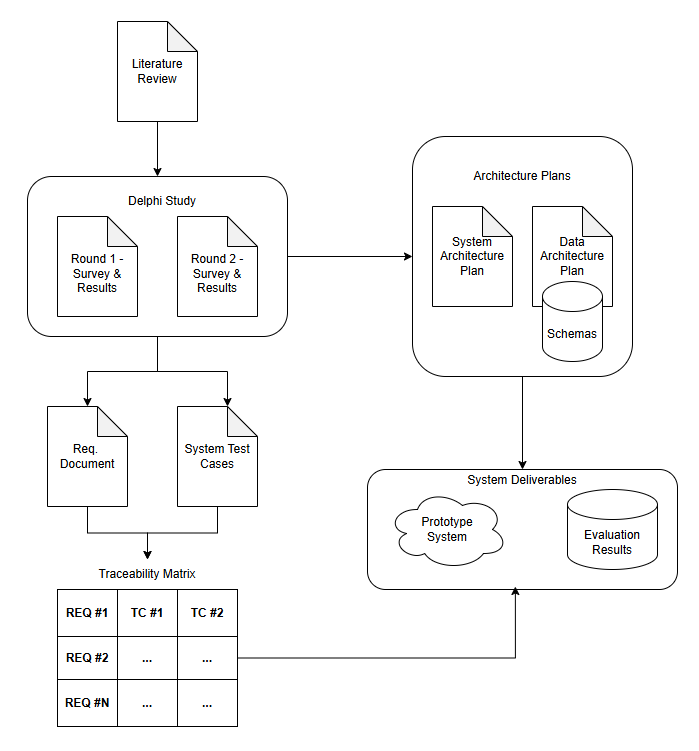
\includegraphics[scale=0.70]{graphic/deliverable_plan.png}}
\caption{Flowchart of Project Deliverables}
\label{fig:deliverable-plan}
\end{figure}

% Perforce software's definition of a Requirements Traceability Matrix --> https://www.perforce.com/resources/alm/requirements-traceability-matrix

These deliverables shall be joined together to form a software system (for which a domain-specific language is the primary user interface). To aid in drawing quantitative conclusions from this system, the researcher plans to develop a \textit{traceability matrix} from the requirements contained in the functional requirements document (FRD). This matrix will be joined to the test cases (TC) that are crafted directly from the requirements in the FRD. 

There is precedent for the use of a traceability matrix when evaluating prototypical software. Yanbin Ye, a previous student of the UA Little Rock Department of Information Science, utilized this approach in \textit{A Positive Data Control System for the Automation of Data Governance Functions}. Ye’s research identified a table of ten (10) system conditions that should be considered in the development of a data control system \cite{yanbin-ye}. Ye then evaluated this prototype to determine how closely the artifact conformed to those requirements. 

Such a scheme for system evaluation is advantageous because it helps to calculate overall system scores--- which are useful when determining if such a software application meets the needs of the intended user base. These scores are often used in information quality settings where quality is gauged on a percentage basis.

As an example, a metric that may be computed during the prototype evaluation is a \textit{conformance score} of the number of test cases that pass for a given requirement (e.g. requirement ID \textit{R1.0.0}). This example is illustrated by the following equation:

\[
\text{Conformance Score}_{\text{R1.0.0}} = 
\frac{\text{\# Test Cases Passed}}{\text{\# Total Test Cases}} 
\times 100\%
\]

Another possible evaluation score is the number of test cycles completed to ensure that all test cases pass for a specific requirement. This evaluation scheme is also helpful because the designer can justify why certain requirements may have been changed (or removed) during the design and development phases of this project.

This traceability matrix is intended to be completed in concert with the requirements document, which is ultimately dependent on the completion of the Delphi study. The requirements modeling and traceability matrix are planned to be completed in the Fall 2025 semester.

%%%%%%%%%%%%%%%%%%%%%%%%%%%%%%%%%%%%%%%%%%%%%%%%%%%%
%
%  New template code for TAMU Theses and Dissertations starting Spring 2021.  
%
%
%  Author: Thesis Office
%  
%  Last Updated: 1/13/2021
%
%%%%%%%%%%%%%%%%%%%%%%%%%%%%%%%%%%%%%%%%%%%%%%%%%%%
%%%%%%%%%%%%%%%%%%%%%%%%%%%%%%%%%%%%%%%%%%%%%%%%%%%%%%%%%%%%%%%%%%%%%%
%%                           SECTION III
%%%%%%%%%%%%%%%%%%%%%%%%%%%%%%%%%%%%%%%%%%%%%%%%%%%%%%%%%%%%%%%%%%%%%

\chapter{\MakeUppercase{Requirements Modeling and Analysis}}
\label{cha:requirements}

This section to discuss the Delphi study conducted as part of this research, along with requirements modeling and analysis.
%%%%%%%%%%%%%%%%%%%%%%%%%%%%%%%%%%%%%%%%%%%%%%%%%%%%
%
%  New template code for TAMU Theses and Dissertations starting Spring 2021.  
%
%
%  Author: Thesis Office
%  
%  Last Updated: 1/13/2021
%
%%%%%%%%%%%%%%%%%%%%%%%%%%%%%%%%%%%%%%%%%%%%%%%%%%%
%%%%%%%%%%%%%%%%%%%%%%%%%%%%%%%%%%%%%%%%%%%%%%%%%%%%%%%%%%%%%%%%%%%%%%
%%                           SECTION IV
%%%%%%%%%%%%%%%%%%%%%%%%%%%%%%%%%%%%%%%%%%%%%%%%%%%%%%%%%%%%%%%%%%%%%



\chapter{SUMMARY AND CONCLUSIONS \label{cha:Summary}}

%%%%%%%%%%%%%%%%%%%%%%%%%%%%%%%%%%%%%%%%%%%%%%%%%%%%
%
%  New template code for TAMU Theses and Dissertations starting Spring 2021.  
%
%
%  Author: Thesis Office
%  
%  Last Updated: 1/13/2021
%
%%%%%%%%%%%%%%%%%%%%%%%%%%%%%%%%%%%%%%%%%%%%%%%%%%%
%%%%%%%%%%%%%%%%%%%%%%%%%%%%%%%%%%%%%%%%%%%%%%%%%%%%%%%%%%%%%%%%%%%%%%
%%                           SECTION V
%%%%%%%%%%%%%%%%%%%%%%%%%%%%%%%%%%%%%%%%%%%%%%%%%%%%%%%%%%%%%%%%%%%%%

\chapter{\MakeUppercase{Implementation}}
\label{cha:implementation}

This chapter is to focus on Implementation details of the system. Including: source code components, parser implementation, web application screenshots, and system evaluation
%%%%%%%%%%%%%%%%%%%%%%%%%%%%%%%%%%%%%%%%%%%%%%%%%%%%
%
%  New template code for TAMU Theses and Dissertations starting Spring 2021.  
%
%
%  Author: Thesis Office
%  
%  Last Updated: 1/13/2021
%
%%%%%%%%%%%%%%%%%%%%%%%%%%%%%%%%%%%%%%%%%%%%%%%%%%%
%%%%%%%%%%%%%%%%%%%%%%%%%%%%%%%%%%%%%%%%%%%%%%%%%%%%%%%%%%%%%%%%%%%%%%
%%                           SECTION VI
%%%%%%%%%%%%%%%%%%%%%%%%%%%%%%%%%%%%%%%%%%%%%%%%%%%%%%%%%%%%%%%%%%%%%

\chapter{\MakeUppercase{Conclusion and Future Work}}
\label{cha:conclusion}

This chapter is to focus on the conclusion of this dissertation. This includes discussion of results found during the evaluation cycle, possible future enhancements that can be made to this system, and any possible future work that can be extended from this platform.
%\include{data/section9}

%The next line is the format for inserting new sections.
%Replace the name "newsection"  with the name of your
%new section file.
%\include{data/newsection}

%fix spacing in bibliography, if any...
%%%%%%%%%%%%%%%%%%%%%%%%%%%%%%%%%%%%%%%%%%%%%%%%%%%%%%%%%%%%%
\let\oldbibitem\bibitem
\renewcommand{\bibitem}{\setlength{\itemsep}{0pt}\oldbibitem}
%%%%%%%%%%%%%%%%%%%%%%%%%%%%%%%%%%%%%%%%%%%%%%%%%%%%%%%%%%%%%%%
%The bibliography style declared is the IEEE format. If
%you require a different style, see the document
%bibstyles.pdf included in this package. This file,
%hosted by the University of Vienna, shows several
%bibliography styles and examples of in-text citation
%and a references page.
%\bibliographystyle{ieeetr}

\phantomsection
\addcontentsline{toc}{chapter}{\numberline{4.}REFERENCES}

\renewcommand{\bibname}{{\normalsize\rm REFERENCES}}

%This file is a .bib database that contains the sources.
%This removes the dependency on the previous file
%bibliography.tex.

\begingroup
\fussy
\raggedright
\bibliographystyle{ieeetr}
\bibliography{data/myReference}
\endgroup




%This next line includes appendices. The file
%appendix.tex contains commands pointing to
%the appendix files; be sure to change these
%pointers if you end up changing the filenames.
%Leave this commented if you will not need
%appendix material.
%%%%%%%%%%%%%%%%%%%%%%%%%%%%%%%%%%%%%%%%%%%%%%%%%%%
%
%  New template code for TAMU Theses and Dissertations starting Spring 2021.  
%
%
%  Author: Thesis Office
%  
%  Last Updated: 1/13/2021
%
%%%%%%%%%%%%%%%%%%%%%%%%%%%%%%%%%%%%%%%%%%%%%%%%%%%

\begin{appendices}
\titleformat{\chapter}{\centering\normalsize}{APPENDIX \thechapter}{0em}{\vskip .5\baselineskip\centering}
\renewcommand{\appendixname}{APPENDIX}

%%%%%%%%%%%%%%%%%%%%%%%%%%%%%%%%%%%%%%%%%%%%%%%%%%%
%
%  New template code for TAMU Theses and Dissertations starting Spring 2021.
%
%
%  Author: Thesis Office 
%	 
%  Last updated 1/13/2021
%
%%%%%%%%%%%%%%%%%%%%%%%%%%%%%%%%%%%%%%%%%%%%%%%%%%%

%%%%%%%%%%%%%%%%%%%%%%%%%%%%%%%%%%%%%%%%%%%%%%%%%%%%%%%%%%%%%%%%%%%%%%
%%                           APPENDIX A 
%%%%%%%%%%%%%%%%%%%%%%%%%%%%%%%%%%%%%%%%%%%%%%%%%%%%%%%%%%%%%%%%%%%%%

\phantomsection

\chapter{\uppercase{Institutional Review Board Certificates}}\label{appendix:A}

\begin{figure}[h]
\centering
\fbox{
\includegraphics[scale=0.55]{figures/irb-approval-letter-1.png}}
\caption{Interview Pilot Study}
\end{figure}

\pagebreak{}

\begin{figure}[h]
\centering
%\fbox{
\includegraphics[scale=0.55]{figures/irb-approval-letter-1.png}}
\fbox{
\includegraphics[scale=0.80]{figures/irb-delphi.png}}
\caption{Delphi Study}
\end{figure}

\pagebreak{}

\begin{figure}[h]
\centering
\fbox{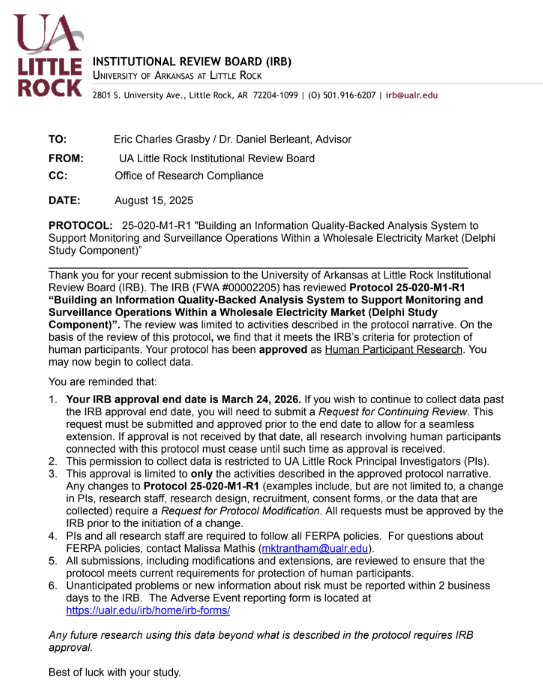
\includegraphics[scale=0.98]{figures/delphi-round-2-irb.png}}
\caption{Delphi Study - Round 2 Protocol Revision}
\end{figure}

%%%%%%%%%%%%%%%%%%%%%%%%%%%%%%%%%%%%%%%%%%%%%%%%%%%
%
%  New template code for TAMU Theses and Dissertations starting Spring 2021.
%
%
%  Author: Thesis Office 
%	 
%  Last updated 1/13/2021
%
%%%%%%%%%%%%%%%%%%%%%%%%%%%%%%%%%%%%%%%%%%%%%%%%%%%

%%%%%%%%%%%%%%%%%%%%%%%%%%%%%%%%%%%%%%%%%%%%%%%%%%%%%%%%%%%%%%%%%%%%%%
%%                           APPENDIX B
%%%%%%%%%%%%%%%%%%%%%%%%%%%%%%%%%%%%%%%%%%%%%%%%%%%%%%%%%%%%%%%%%%%%%


\chapter{\uppercase {Search Queries used in Literature Review}}\label{appendix:B}

\noindent \textit{Google Scholar and IEEE Xplore were the primary academic databases that were queried for this dissertation.}
\newline

\noindent High-level searches used to find seminal articles in the areas of energy markets, market monitoring, and domain-specific languages:

\begin{itemize}
    \item \MakeUppercase{Market Monitoring}
    \item \MakeUppercase{Market Monitoring and Domain Specific Language}
    \item \MakeUppercase{Domain-Specific Language and Bulk Electric System}
    \item \MakeUppercase{Domain Specific Language and Forensics}
    \item \MakeUppercase{Domain-Specific Language}
\end{itemize}

\noindent Boolean and grouping operators were also employed to narrow the scope of the relevant articles returned for this literature review. Some of the queries included: 

\begin{itemize}
    \item \MakeUppercase{"MARKET MONITORING" AND ("DOMAIN SPECIFIC LANGUAGE" OR "DOMAIN-SPECIFIC LANGUAGE")}
    \item \MakeUppercase{"MARKET MONITORING" AND ("DOMAIN SPECIFIC LANGUAGE" OR "DOMAIN-SPECIFIC LANGUAGE") AND ("ELECTRIC" OR "ELECTRICITY") -stock}
    \item \MakeUppercase{("INFORMATION QUALITY" OR "DATA QUALITY") ("ELECTRICITY MARKET" OR "POWER MARKET" OR "ELECTRIC MARKET")}
    \item \MakeUppercase{("INFORMATION QUALITY" OR "DATA QUALITY") (ELECTRICITY OR POWER OR ELECTRIC OR ENERGY) MARKET}
    \item \MakeUppercase{("INFORMATION QUALITY" OR "DATA QUALITY") (ELECTRICITY OR POWER OR ELECTRIC OR ENERGY) "MARKET MONITORING"}
    \item \MakeUppercase{("INFORMATION QUALITY" OR "DATA QUALITY") (ELECTRICITY OR POWER OR ELECTRIC OR ENERGY) WHOLESALE "MARKET MONITORING" -labor -labour -"financial market"}
    \item \MakeUppercase{allintitle: WHOLESALE "INFORMATION QUALITY" OR "DATA QUALITY" OR ELECTRICITY OR POWER OR ELECTRIC OR ENERGY "MARKET MONITORING" -labor -labour -"financial market"}
    \item \MakeUppercase{allintitle: ELECTRICITY "INFORMATION QUALITY" OR "DATA QUALITY" OR "MARKET MONITORING" -labor -labour
    ("DOMAIN-SPECIFIC LANGUAGE" OR "DOMAIN SPECIFIC LANGUAGE") (ELECTRICITY OR ELECTRIC OR POWER OR ENERGY)}
    
\end{itemize}


\pagebreak{}

\phantomsection

\chapter{\uppercase{Schedule of Research Milestones}}\label{appendix:C}

\let\mc=\multicolumn
\let\mr=\multirow
\let\cl=\cline

\noindent Note that these milestones are subject to change by the discretion of the principal investigator and research advisor. The timeline may change as milestones are completed.
\begin{center}
\begin{table}[ht]
    \centering
    \begin{tabular}{|c|c|c|}
        \hline
        \mr{1}{*}{\textbf{Semester}} & \textbf{Milestone Description} & \textbf{Associated Deliverables} \\ 
        \cline{1-3}
        \mr{3}{*}{\MakeUppercase{Fall 2024}} & Article Gathering for Literature Review & \textit{Retrieved Existing Research} \\ \cline{2-3}
        & Literature Review Interviews & \textit{Interview Results} \\ \cline{2-3}
        & Preparation for Qualifying Exam & \textit{Slide Deck and Summary} \\ \cline{2-3}
        & Complete Qualifying Exam & --- \\ \cline{2-3}
        & Complete Required CITI Modules & \textit{CITI Completion Certificate(s)} \\ \cline{2-3}
        \hline
        \mr{2}{*}{\MakeUppercase{Spring 2025}} & Complete Writing Literature Review & \textit{Dissertation Chapter (2)} \\ \cline{2-3}
        & Complete Writing Proposal & \textit{Dissertation Proposal} \\ \cline{2-3}
        & Schedule Proposal Defense & --- \\ \cline{2-3}
        & Complete Proposal Defense & --- \\ \cline{2-3}
        & Develop Initial Set of Delphi Study Questions & \textit{Delphi Study Questions} \\ \cline{2-3}
        & Seek IRB Approval & \textit{IRB Approval Letter} \\ \cline{2-3}
        & Begin Seating Delphi Panel & \textit{Coordination with Experts} \\ 
        \hline
        \mr{2}{*}{\MakeUppercase{Summer 2025}} & Complete Dephi Study & \textit{Paper Publication} \\ \cline{2-3}
        & Create Requirements Document & \textit{FRD, BPMN Flows, etc.} \\ 
        \hline
        \mr{2}{*}{\MakeUppercase{Fall 2025}} & Finish Requirements Chapter & \textit{Dissertation Chapter (3)} \\ \cline{2-3}
        & Begin Prototype Development & \textit{Prototype Artifacts} \\ \cline{2-3}
        & Begin DSL specification & \textit{DSL Spec} \\ \cline{2-3}
        & Begin Implementation Dissertation Chapter & \textit{Dissertation Chapter (4)} \\
        \hline
        \mr{2}{*}{\MakeUppercase{Spring 2026}} & Iterative Development & \textit{Prototype Artifacts (cont)} \\ \cline{2-3}
        & Track evaluation metrics for prototype & \textit{Evaluation results} \\ 
        \hline
        \mr{2}{*}{\MakeUppercase{Summer 2026}} & Prototype Setup/Deployment & \textit{PoC environment} \\ \cline{2-3}
        & Iterative Development \& Bugfixes & \textit{Bug-fixes / version enhancements} \\ \cline{2-3}
        & Implementation and Evaluation Chapters & \textit{Dissertation Chapters (4, 5)} \\
        \hline
        \mr{2}{*}{\MakeUppercase{Fall 2026}} & Finish Conclusion Chapter & \textit{Dissertation Chapter (6)} \\ \cline{2-3}
        & Complete Dissertation Formatting & \textit{Dissertation Ready for Defense} \\ \cline{2-3}
        & Dissertation Defense & --- \\
        \hline
    \end{tabular}
    \caption{Schedule of Milestones for this Dissertation}
    \label{tab:example}
\end{table}
\end{center}
%%%%%%%%%%%%%%%%%%%%%%%%%%%%%%%%%%%%%%%%%%%%%%%%%%%%
%
%  New template code for TAMU Theses and Dissertations starting Spring 2021.
%
%
%  Author: Thesis Office 
%	 
%  Last updated 1/13/2021
%
%%%%%%%%%%%%%%%%%%%%%%%%%%%%%%%%%%%%%%%%%%%%%%%%%%%

%%%%%%%%%%%%%%%%%%%%%%%%%%%%%%%%%%%%%%%%%%%%%%%%%%%%%%%%%%%%%%%%%%%%%%
%%                           APPENDIX D
%%%%%%%%%%%%%%%%%%%%%%%%%%%%%%%%%%%%%%%%%%%%%%%%%%%%%%%%%%%%%%%%%%%%%


\chapter{\uppercase {Prototype Version History}}\label{appendix:D}

\noindent \textbf{Domain-Specific Language Specification ("FILTER")}
\newline

\begin{itemize}
    \item \MakeUppercase{VERSION 2025-03-11}
\end{itemize}

\noindent \textbf{Web Application}
\newline

\begin{itemize}
    \item \MakeUppercase{VERSION 2025-03-11}
\end{itemize}
\pagebreak{}
%%%%%%%%%%%%%%%%%%%%%%%%%%%%%%%%%%%%%%%%%%%%%%%%%%%%%%%%%%%%%%%%%%%%%%%%%%%%%%%%%%%
%   APPENDIX 5 - 
%%%%%%%%%%%%%%%%%%%%%%%%%%%%%%%%%%%%%%%%%%%%%%%%%%%%%%%%%%%%%%%%%%%%%%%%%%%%%%%%%%%

\chapter{\uppercase {Public Market Data Sources}}\label{appendix:E}

\begin{itemize}
    \item Data Miner 2, PJM Corporation - \url{https://dataminer2.pjm.com/list}
    \item Member Information Reporting Application (MIRA), Monitoring Analytics - \\ \url{https://www.monitoringanalytics.com/tools/tools.shtml}
    \item Market Data Transparency Service, ERCOT - \\ \url{https://www.ercot.com/services/mdt}
    \item Open Access Same-Time Information System, California ISO - \\ \url{http://oasis.caiso.com/mrioasis/logon.do}
    \item CAISO Data Library, California ISO - \\ \url{https://www.caiso.com/library/market-data}
    \item MISO Data Exchange, MISO - \url{https://data-exchange.misoenergy.org/}
    \item Marketplace Portal, Southwest Power Pool - \url{https://portal.spp.org/}
    \item Wholesale Energy Market Reports, US Energy Information Administration (EIA) - \\ \url{https://www.eia.gov/electricity/}
    \item Operational Data Portal, New York ISO - \\ \url{https://www.nyiso.com/energy-market-operational-data}
    \item ISO Express, ISO New England - \\ \url{https://www.iso-ne.com/markets-operations/iso-express}
\end{itemize}

\begin{figure}[H]
\centering
\fbox{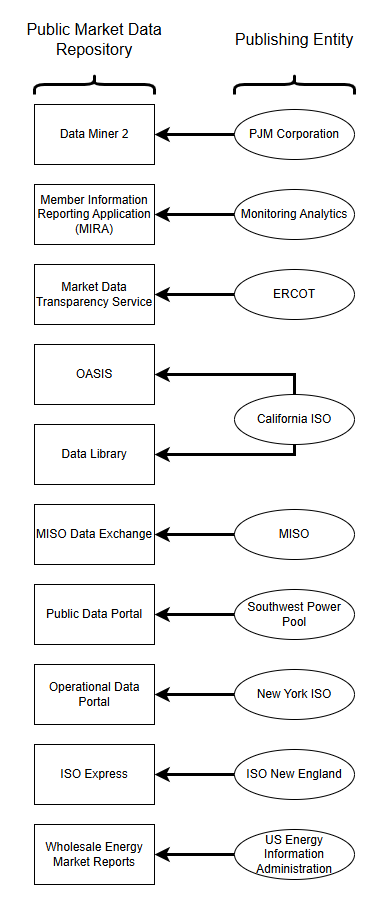
\includegraphics[scale=0.85]{graphic/market-comps.png}}
\caption{Public Market Data Sources}
\label{fig:market-comps}
\end{figure}

\end{appendices}


\end{document}
